\documentclass[11pt]{beamer}

\usepackage[utf8]{inputenc}
\usepackage[english]{babel}
\usepackage{amsmath}
\usepackage{amsfonts}
\usepackage{amssymb}
\usepackage{tikz}
\author[shortname]{Domagoj Fizulic \and Felix Gutmann}

\title{Unsupervised Learning in Decision Making}
%\setbeamercovered{transparent} 
%\setbeamertemplate{navigation symbols}{} 
%\logo{} 
%\institute{} 
%\date{} 
\subject{Master Project} 
\begin{document}
	
\frame{\titlepage}

\begin{frame}{Introduction}
\setbeamertemplate{itemize items}[circle]
\begin{itemize}
	\item Introduction
	\item Reinforcement learning and simulation
	\item Experiment Data 
	\item Experiment results
\end{itemize}
\end{frame}
	
\begin{frame}{Reinforcement Learning}
	\framesubtitle{Multi arm bandit experiment}
	\setbeamertemplate{itemize items}[circle]
	\begin{figure}
		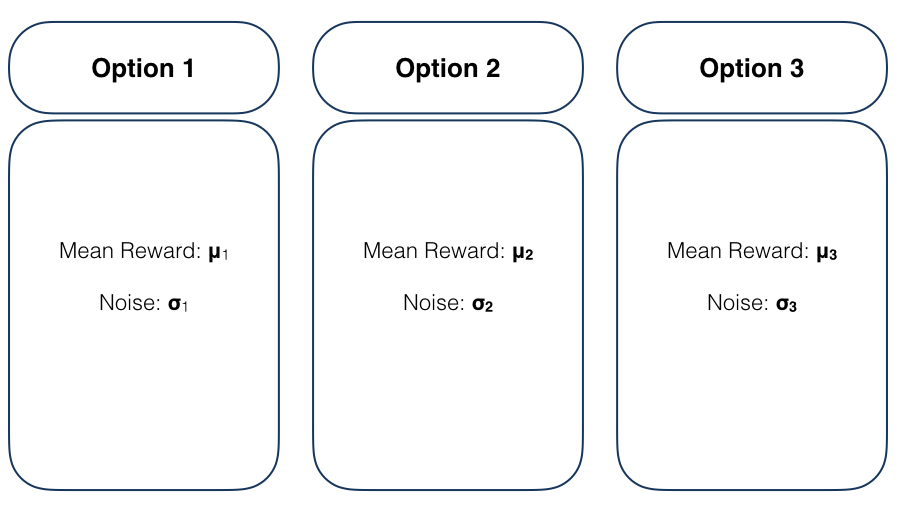
\includegraphics[scale=0.3]{Pictures/p2.png}
	\end{figure}

	\begin{itemize}
		\item Choose sequentially from set of choices 
		\item Objective: Maximize revenues
	\end{itemize}
\end{frame}

\begin{frame}{Reinforcement Learning}
\setbeamertemplate{itemize items}[circle]
\framesubtitle{Essential functions and agent modeling}
Softmax Decision Function:
\begin{align*}
P(a)_{t+1} &= \frac{e^{\frac{Q_t(a)}{\tau}}}{\sum_{i}^{N} e^{\frac{Q_t(i)}{\tau}}}
\intertext{Update rule for value function of an action:}
Q(a)_{t+1} &= Q(a)_t + \alpha \left[ R(a)_t -  Q(a)_t	 \right]
\end{align*}
where
\begin{itemize}
	\item $Q(a)$ is the value function of action $a$
	\item $R(a)$ is the reward for action $a$
	\item $\tau$ is the \textit{"temparature"}, controlling randomised behaviour
	\item $\alpha$ is the learning rate ($\alpha \in [0,1]$)
\end{itemize}

\end{frame}

\begin{frame}{Reinforcement Learning}
	\framesubtitle{Experiment design and simulation results}
	\setbeamertemplate{itemize items}[circle]
	\hspace*{-0.06in}
	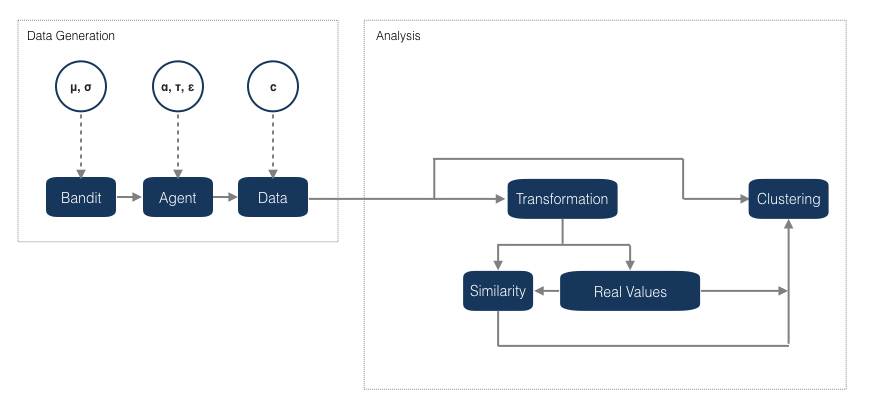
\includegraphics[scale=0.35]{Pictures/f2.jpeg}
	
		Key - findings:
		\begin{itemize}
			\item Clustering based on $\tau$ differences possible ($\Delta \approx 0.7$) 
			\item Clustering based on $\alpha$ difficult. Good clustering only with very high differences ($\Delta \approx 0.99$)
		\end{itemize} 
\end{frame}


\begin{frame}{Data Analysis}
	\framesubtitle{Analysed data sets}
	\setbeamertemplate{itemize items}[circle]
	
	\textbf{20-Arm Bandit Experiment:}
	\begin{itemize}
		\item Four experiment types with different means and noises
		\item 429 participants 
	\end{itemize} 
	
	\textbf{Data based on Iowa Gambling Task }
	\begin{itemize}
		\item IGT data for 96 participants with 11 criminal profiles
		\item IGT for cocaine abusers
	\end{itemize} 
\end{frame}

\begin{frame}{Experiment Results}
	\framesubtitle{Multi arm bandit experiments}
	\setbeamertemplate{itemize items}[circle]
	
	\begin{itemize}
		\item Use data to estimate clusters 
		\item Estimated parameters from soft max equation using numerical optimization
		\item Try to see if unsupervised learning is recovering results from cognitive science
	\end{itemize}

\end{frame}

\begin{frame}{Experiment Results}
	\framesubtitle{Multi arm bandit experiments - 2 Clusters / Spectral RBF / Blockwise Entropy}
	\setbeamertemplate{itemize items}[circle]
		\center
		% Created by tikzDevice version 0.10.1 on 2016-06-29 14:17:03
% !TEX encoding = UTF-8 Unicode
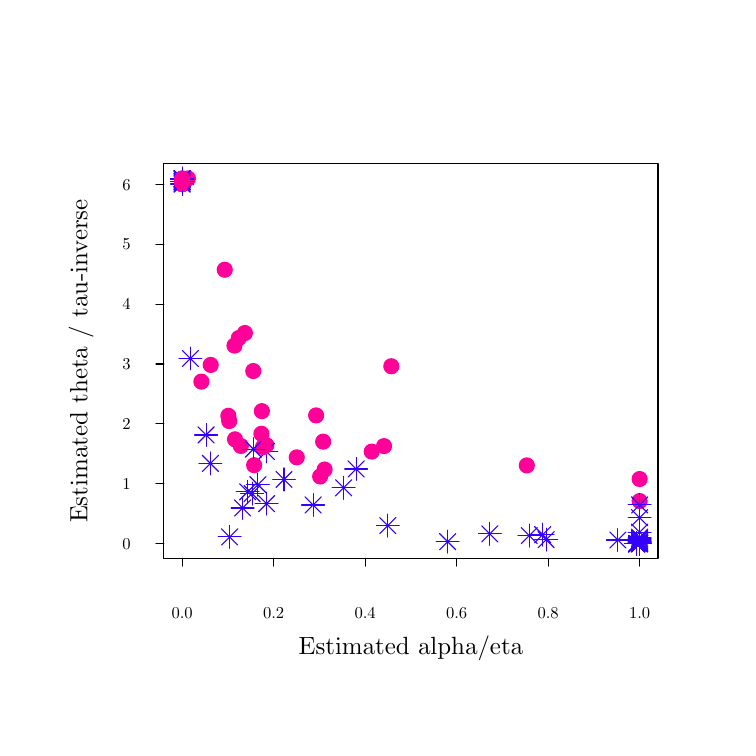
\begin{tikzpicture}[x=1pt,y=1pt]
\definecolor{fillColor}{RGB}{255,255,255}
\path[use as bounding box,fill=fillColor,fill opacity=0.00] (0,0) rectangle (252.94,252.94);
\begin{scope}
\path[clip] ( 49.20, 61.20) rectangle (227.75,203.75);
\definecolor{drawColor}{RGB}{51,0,255}

\path[draw=drawColor,line width= 0.4pt,line join=round,line cap=round] (218.21, 67.70) -- (224.06, 73.55);

\path[draw=drawColor,line width= 0.4pt,line join=round,line cap=round] (218.21, 73.55) -- (224.06, 67.70);

\path[draw=drawColor,line width= 0.4pt,line join=round,line cap=round] (216.99, 70.63) -- (225.27, 70.63);

\path[draw=drawColor,line width= 0.4pt,line join=round,line cap=round] (221.13, 66.49) -- (221.13, 74.77);

\path[draw=drawColor,line width= 0.4pt,line join=round,line cap=round] (218.21, 64.53) -- (224.06, 70.38);

\path[draw=drawColor,line width= 0.4pt,line join=round,line cap=round] (218.21, 70.38) -- (224.06, 64.53);

\path[draw=drawColor,line width= 0.4pt,line join=round,line cap=round] (217.00, 67.46) -- (225.27, 67.46);

\path[draw=drawColor,line width= 0.4pt,line join=round,line cap=round] (221.13, 63.32) -- (221.13, 71.59);

\path[draw=drawColor,line width= 0.4pt,line join=round,line cap=round] (217.14, 63.55) -- (222.99, 69.40);

\path[draw=drawColor,line width= 0.4pt,line join=round,line cap=round] (217.14, 69.40) -- (222.99, 63.55);

\path[draw=drawColor,line width= 0.4pt,line join=round,line cap=round] (215.93, 66.48) -- (224.21, 66.48);

\path[draw=drawColor,line width= 0.4pt,line join=round,line cap=round] (220.07, 62.34) -- (220.07, 70.62);
\definecolor{fillColor}{RGB}{255,0,153}

\path[fill=fillColor] ( 55.81,196.36) circle (  2.92);

\path[draw=drawColor,line width= 0.4pt,line join=round,line cap=round] ( 52.89,193.48) -- ( 58.74,199.33);

\path[draw=drawColor,line width= 0.4pt,line join=round,line cap=round] ( 52.89,199.33) -- ( 58.74,193.48);

\path[draw=drawColor,line width= 0.4pt,line join=round,line cap=round] ( 51.68,196.40) -- ( 59.95,196.40);

\path[draw=drawColor,line width= 0.4pt,line join=round,line cap=round] ( 55.81,192.27) -- ( 55.81,200.54);

\path[fill=fillColor] (221.13, 81.89) circle (  2.92);

\path[fill=fillColor] ( 55.81,197.86) circle (  2.92);

\path[fill=fillColor] ( 55.81,197.47) circle (  2.92);

\path[fill=fillColor] ( 55.81,197.08) circle (  2.92);

\path[fill=fillColor] ( 77.02,101.80) circle (  2.92);

\path[fill=fillColor] ( 78.50,142.61) circle (  2.92);

\path[draw=drawColor,line width= 0.4pt,line join=round,line cap=round] ( 52.89,195.14) -- ( 58.74,200.99);

\path[draw=drawColor,line width= 0.4pt,line join=round,line cap=round] ( 52.89,200.99) -- ( 58.74,195.14);

\path[draw=drawColor,line width= 0.4pt,line join=round,line cap=round] ( 51.68,198.07) -- ( 59.95,198.07);

\path[draw=drawColor,line width= 0.4pt,line join=round,line cap=round] ( 55.81,193.93) -- ( 55.81,202.20);

\path[fill=fillColor] (221.13, 89.84) circle (  2.92);

\path[draw=drawColor,line width= 0.4pt,line join=round,line cap=round] (184.42, 65.01) -- (190.27, 70.86);

\path[draw=drawColor,line width= 0.4pt,line join=round,line cap=round] (184.42, 70.86) -- (190.27, 65.01);

\path[draw=drawColor,line width= 0.4pt,line join=round,line cap=round] (183.21, 67.94) -- (191.49, 67.94);

\path[draw=drawColor,line width= 0.4pt,line join=round,line cap=round] (187.35, 63.80) -- (187.35, 72.07);

\path[fill=fillColor] ( 84.62,114.37) circle (  2.92);

\path[fill=fillColor] (106.77,103.34) circle (  2.92);

\path[fill=fillColor] (107.29, 93.27) circle (  2.92);

\path[fill=fillColor] ( 55.81,196.52) circle (  2.92);

\path[fill=fillColor] ( 86.26,102.07) circle (  2.92);

\path[draw=drawColor,line width= 0.4pt,line join=round,line cap=round] (218.21, 64.28) -- (224.06, 70.13);

\path[draw=drawColor,line width= 0.4pt,line join=round,line cap=round] (218.21, 70.13) -- (224.06, 64.28);

\path[draw=drawColor,line width= 0.4pt,line join=round,line cap=round] (217.00, 67.20) -- (225.27, 67.20);

\path[draw=drawColor,line width= 0.4pt,line join=round,line cap=round] (221.13, 63.07) -- (221.13, 71.34);

\path[draw=drawColor,line width= 0.4pt,line join=round,line cap=round] (218.09, 63.55) -- (223.94, 69.40);

\path[draw=drawColor,line width= 0.4pt,line join=round,line cap=round] (218.09, 69.40) -- (223.94, 63.55);

\path[draw=drawColor,line width= 0.4pt,line join=round,line cap=round] (216.88, 66.48) -- (225.15, 66.48);

\path[draw=drawColor,line width= 0.4pt,line join=round,line cap=round] (221.01, 62.34) -- (221.01, 70.62);

\path[draw=drawColor,line width= 0.4pt,line join=round,line cap=round] ( 89.70, 86.76) -- ( 95.55, 92.61);

\path[draw=drawColor,line width= 0.4pt,line join=round,line cap=round] ( 89.70, 92.61) -- ( 95.55, 86.76);

\path[draw=drawColor,line width= 0.4pt,line join=round,line cap=round] ( 88.49, 89.69) -- ( 96.76, 89.69);

\path[draw=drawColor,line width= 0.4pt,line join=round,line cap=round] ( 92.63, 85.55) -- ( 92.63, 93.82);

\path[draw=drawColor,line width= 0.4pt,line join=round,line cap=round] (148.84, 64.28) -- (154.69, 70.13);

\path[draw=drawColor,line width= 0.4pt,line join=round,line cap=round] (148.84, 70.13) -- (154.69, 64.28);

\path[draw=drawColor,line width= 0.4pt,line join=round,line cap=round] (147.63, 67.21) -- (155.90, 67.21);

\path[draw=drawColor,line width= 0.4pt,line join=round,line cap=round] (151.76, 63.07) -- (151.76, 71.34);

\path[draw=drawColor,line width= 0.4pt,line join=round,line cap=round] ( 52.89,194.35) -- ( 58.74,200.20);

\path[draw=drawColor,line width= 0.4pt,line join=round,line cap=round] ( 52.89,200.20) -- ( 58.74,194.35);

\path[draw=drawColor,line width= 0.4pt,line join=round,line cap=round] ( 51.68,197.28) -- ( 59.95,197.28);

\path[draw=drawColor,line width= 0.4pt,line join=round,line cap=round] ( 55.81,193.14) -- ( 55.81,201.41);

\path[draw=drawColor,line width= 0.4pt,line join=round,line cap=round] (218.09, 63.55) -- (223.94, 69.40);

\path[draw=drawColor,line width= 0.4pt,line join=round,line cap=round] (218.09, 69.40) -- (223.94, 63.55);

\path[draw=drawColor,line width= 0.4pt,line join=round,line cap=round] (216.88, 66.48) -- (225.15, 66.48);

\path[draw=drawColor,line width= 0.4pt,line join=round,line cap=round] (221.01, 62.34) -- (221.01, 70.62);

\path[fill=fillColor] (131.39,130.60) circle (  2.92);

\path[fill=fillColor] ( 62.76,125.04) circle (  2.92);

\path[draw=drawColor,line width= 0.4pt,line join=round,line cap=round] (217.14, 63.55) -- (222.99, 69.40);

\path[draw=drawColor,line width= 0.4pt,line join=round,line cap=round] (217.14, 69.40) -- (222.99, 63.55);

\path[draw=drawColor,line width= 0.4pt,line join=round,line cap=round] (215.93, 66.48) -- (224.21, 66.48);

\path[draw=drawColor,line width= 0.4pt,line join=round,line cap=round] (220.07, 62.34) -- (220.07, 70.62);

\path[draw=drawColor,line width= 0.4pt,line join=round,line cap=round] (100.20, 77.54) -- (106.05, 83.39);

\path[draw=drawColor,line width= 0.4pt,line join=round,line cap=round] (100.20, 83.39) -- (106.05, 77.54);

\path[draw=drawColor,line width= 0.4pt,line join=round,line cap=round] ( 98.99, 80.47) -- (107.27, 80.47);

\path[draw=drawColor,line width= 0.4pt,line join=round,line cap=round] (103.13, 76.33) -- (103.13, 84.60);

\path[draw=drawColor,line width= 0.4pt,line join=round,line cap=round] ( 83.30, 96.87) -- ( 89.15,102.72);

\path[draw=drawColor,line width= 0.4pt,line join=round,line cap=round] ( 83.30,102.72) -- ( 89.15, 96.87);

\path[draw=drawColor,line width= 0.4pt,line join=round,line cap=round] ( 82.09, 99.79) -- ( 90.36, 99.79);

\path[draw=drawColor,line width= 0.4pt,line join=round,line cap=round] ( 86.23, 95.66) -- ( 86.23,103.93);

\path[draw=drawColor,line width= 0.4pt,line join=round,line cap=round] (218.09, 63.55) -- (223.94, 69.40);

\path[draw=drawColor,line width= 0.4pt,line join=round,line cap=round] (218.09, 69.40) -- (223.94, 63.55);

\path[draw=drawColor,line width= 0.4pt,line join=round,line cap=round] (216.88, 66.48) -- (225.15, 66.48);

\path[draw=drawColor,line width= 0.4pt,line join=round,line cap=round] (221.01, 62.34) -- (221.01, 70.62);

\path[fill=fillColor] ( 97.23, 97.68) circle (  2.92);

\path[fill=fillColor] ( 72.52,112.69) circle (  2.92);

\path[draw=drawColor,line width= 0.4pt,line join=round,line cap=round] ( 52.89,194.28) -- ( 58.74,200.13);

\path[draw=drawColor,line width= 0.4pt,line join=round,line cap=round] ( 52.89,200.13) -- ( 58.74,194.28);

\path[draw=drawColor,line width= 0.4pt,line join=round,line cap=round] ( 51.68,197.20) -- ( 59.95,197.20);

\path[draw=drawColor,line width= 0.4pt,line join=round,line cap=round] ( 55.81,193.07) -- ( 55.81,201.34);

\path[draw=drawColor,line width= 0.4pt,line join=round,line cap=round] (218.21, 63.55) -- (224.06, 69.40);

\path[draw=drawColor,line width= 0.4pt,line join=round,line cap=round] (218.21, 69.40) -- (224.06, 63.55);

\path[draw=drawColor,line width= 0.4pt,line join=round,line cap=round] (217.00, 66.48) -- (225.27, 66.48);

\path[draw=drawColor,line width= 0.4pt,line join=round,line cap=round] (221.13, 62.34) -- (221.13, 70.62);

\path[fill=fillColor] ( 57.92,198.45) circle (  2.92);

\path[fill=fillColor] ( 85.02,101.38) circle (  2.92);

\path[fill=fillColor] ( 55.81,197.24) circle (  2.92);

\path[draw=drawColor,line width= 0.4pt,line join=round,line cap=round] ( 63.12, 92.55) -- ( 68.97, 98.40);

\path[draw=drawColor,line width= 0.4pt,line join=round,line cap=round] ( 63.12, 98.40) -- ( 68.97, 92.55);

\path[draw=drawColor,line width= 0.4pt,line join=round,line cap=round] ( 61.91, 95.47) -- ( 70.18, 95.47);

\path[draw=drawColor,line width= 0.4pt,line join=round,line cap=round] ( 66.04, 91.34) -- ( 66.04, 99.61);

\path[fill=fillColor] (105.68, 90.77) circle (  2.92);

\path[fill=fillColor] ( 55.81,196.40) circle (  2.92);

\path[draw=drawColor,line width= 0.4pt,line join=round,line cap=round] (217.14, 63.55) -- (222.99, 69.40);

\path[draw=drawColor,line width= 0.4pt,line join=round,line cap=round] (217.14, 69.40) -- (222.99, 63.55);

\path[draw=drawColor,line width= 0.4pt,line join=round,line cap=round] (215.93, 66.48) -- (224.21, 66.48);

\path[draw=drawColor,line width= 0.4pt,line join=round,line cap=round] (220.07, 62.34) -- (220.07, 70.62);

\path[fill=fillColor] ( 76.29,140.79) circle (  2.92);

\path[draw=drawColor,line width= 0.4pt,line join=round,line cap=round] ( 61.54,102.85) -- ( 67.39,108.70);

\path[draw=drawColor,line width= 0.4pt,line join=round,line cap=round] ( 61.54,108.70) -- ( 67.39,102.85);

\path[draw=drawColor,line width= 0.4pt,line join=round,line cap=round] ( 60.33,105.77) -- ( 68.60,105.77);

\path[draw=drawColor,line width= 0.4pt,line join=round,line cap=round] ( 64.47,101.64) -- ( 64.47,109.91);

\path[draw=drawColor,line width= 0.4pt,line join=round,line cap=round] (217.14, 63.55) -- (222.99, 69.40);

\path[draw=drawColor,line width= 0.4pt,line join=round,line cap=round] (217.14, 69.40) -- (222.99, 63.55);

\path[draw=drawColor,line width= 0.4pt,line join=round,line cap=round] (215.93, 66.48) -- (224.21, 66.48);

\path[draw=drawColor,line width= 0.4pt,line join=round,line cap=round] (220.07, 62.34) -- (220.07, 70.62);

\path[draw=drawColor,line width= 0.4pt,line join=round,line cap=round] (111.26, 83.75) -- (117.11, 89.60);

\path[draw=drawColor,line width= 0.4pt,line join=round,line cap=round] (111.26, 89.60) -- (117.11, 83.75);

\path[draw=drawColor,line width= 0.4pt,line join=round,line cap=round] (110.05, 86.68) -- (118.32, 86.68);

\path[draw=drawColor,line width= 0.4pt,line join=round,line cap=round] (114.19, 82.54) -- (114.19, 90.81);

\path[draw=drawColor,line width= 0.4pt,line join=round,line cap=round] ( 74.74, 76.46) -- ( 80.59, 82.31);

\path[draw=drawColor,line width= 0.4pt,line join=round,line cap=round] ( 74.74, 82.31) -- ( 80.59, 76.46);

\path[draw=drawColor,line width= 0.4pt,line join=round,line cap=round] ( 73.53, 79.39) -- ( 81.80, 79.39);

\path[draw=drawColor,line width= 0.4pt,line join=round,line cap=round] ( 77.67, 75.25) -- ( 77.67, 83.52);

\path[draw=drawColor,line width= 0.4pt,line join=round,line cap=round] ( 52.89,195.31) -- ( 58.74,201.16);

\path[draw=drawColor,line width= 0.4pt,line join=round,line cap=round] ( 52.89,201.16) -- ( 58.74,195.31);

\path[draw=drawColor,line width= 0.4pt,line join=round,line cap=round] ( 51.68,198.24) -- ( 59.95,198.24);

\path[draw=drawColor,line width= 0.4pt,line join=round,line cap=round] ( 55.81,194.10) -- ( 55.81,202.37);

\path[draw=drawColor,line width= 0.4pt,line join=round,line cap=round] (217.14, 63.55) -- (222.99, 69.40);

\path[draw=drawColor,line width= 0.4pt,line join=round,line cap=round] (217.14, 69.40) -- (222.99, 63.55);

\path[draw=drawColor,line width= 0.4pt,line join=round,line cap=round] (215.93, 66.48) -- (224.21, 66.48);

\path[draw=drawColor,line width= 0.4pt,line join=round,line cap=round] (220.07, 62.34) -- (220.07, 70.62);

\path[fill=fillColor] ( 55.81,197.55) circle (  2.92);

\path[fill=fillColor] ( 66.14,131.07) circle (  2.92);

\path[draw=drawColor,line width= 0.4pt,line join=round,line cap=round] ( 78.17, 81.66) -- ( 84.02, 87.51);

\path[draw=drawColor,line width= 0.4pt,line join=round,line cap=round] ( 78.17, 87.51) -- ( 84.02, 81.66);

\path[draw=drawColor,line width= 0.4pt,line join=round,line cap=round] ( 76.96, 84.59) -- ( 85.23, 84.59);

\path[draw=drawColor,line width= 0.4pt,line join=round,line cap=round] ( 81.10, 80.45) -- ( 81.10, 88.72);

\path[fill=fillColor] ( 55.81,198.47) circle (  2.92);

\path[draw=drawColor,line width= 0.4pt,line join=round,line cap=round] (178.32, 66.48) -- (184.17, 72.33);

\path[draw=drawColor,line width= 0.4pt,line join=round,line cap=round] (178.32, 72.33) -- (184.17, 66.48);

\path[draw=drawColor,line width= 0.4pt,line join=round,line cap=round] (177.11, 69.41) -- (185.38, 69.41);

\path[draw=drawColor,line width= 0.4pt,line join=round,line cap=round] (181.25, 65.27) -- (181.25, 73.54);

\path[fill=fillColor] ( 81.52,128.87) circle (  2.92);

\path[fill=fillColor] ( 71.21,165.47) circle (  2.92);

\path[draw=drawColor,line width= 0.4pt,line join=round,line cap=round] ( 52.89,194.34) -- ( 58.74,200.19);

\path[draw=drawColor,line width= 0.4pt,line join=round,line cap=round] ( 52.89,200.19) -- ( 58.74,194.34);

\path[draw=drawColor,line width= 0.4pt,line join=round,line cap=round] ( 51.68,197.27) -- ( 59.95,197.27);

\path[draw=drawColor,line width= 0.4pt,line join=round,line cap=round] ( 55.81,193.13) -- ( 55.81,201.40);

\path[draw=drawColor,line width= 0.4pt,line join=round,line cap=round] ( 52.89,195.48) -- ( 58.74,201.33);

\path[draw=drawColor,line width= 0.4pt,line join=round,line cap=round] ( 52.89,201.33) -- ( 58.74,195.48);

\path[draw=drawColor,line width= 0.4pt,line join=round,line cap=round] ( 51.68,198.41) -- ( 59.95,198.41);

\path[draw=drawColor,line width= 0.4pt,line join=round,line cap=round] ( 55.81,194.27) -- ( 55.81,202.55);

\path[draw=drawColor,line width= 0.4pt,line join=round,line cap=round] (218.21, 77.56) -- (224.06, 83.41);

\path[draw=drawColor,line width= 0.4pt,line join=round,line cap=round] (218.21, 83.41) -- (224.06, 77.56);

\path[draw=drawColor,line width= 0.4pt,line join=round,line cap=round] (217.00, 80.48) -- (225.27, 80.48);

\path[draw=drawColor,line width= 0.4pt,line join=round,line cap=round] (221.13, 76.35) -- (221.13, 84.62);

\path[draw=drawColor,line width= 0.4pt,line join=round,line cap=round] ( 76.56, 82.29) -- ( 82.41, 88.14);

\path[draw=drawColor,line width= 0.4pt,line join=round,line cap=round] ( 76.56, 88.14) -- ( 82.41, 82.29);

\path[draw=drawColor,line width= 0.4pt,line join=round,line cap=round] ( 75.35, 85.21) -- ( 83.62, 85.21);

\path[draw=drawColor,line width= 0.4pt,line join=round,line cap=round] ( 79.48, 81.08) -- ( 79.48, 89.35);

\path[draw=drawColor,line width= 0.4pt,line join=round,line cap=round] (218.21, 64.13) -- (224.06, 69.98);

\path[draw=drawColor,line width= 0.4pt,line join=round,line cap=round] (218.21, 69.98) -- (224.06, 64.13);

\path[draw=drawColor,line width= 0.4pt,line join=round,line cap=round] (217.00, 67.06) -- (225.27, 67.06);

\path[draw=drawColor,line width= 0.4pt,line join=round,line cap=round] (221.13, 62.92) -- (221.13, 71.19);

\path[fill=fillColor] ( 74.92,104.19) circle (  2.92);

\path[draw=drawColor,line width= 0.4pt,line join=round,line cap=round] (218.21, 63.55) -- (224.06, 69.40);

\path[draw=drawColor,line width= 0.4pt,line join=round,line cap=round] (218.21, 69.40) -- (224.06, 63.55);

\path[draw=drawColor,line width= 0.4pt,line join=round,line cap=round] (217.00, 66.48) -- (225.27, 66.48);

\path[draw=drawColor,line width= 0.4pt,line join=round,line cap=round] (221.13, 62.34) -- (221.13, 70.62);

\path[draw=drawColor,line width= 0.4pt,line join=round,line cap=round] ( 70.05, 65.99) -- ( 75.90, 71.84);

\path[draw=drawColor,line width= 0.4pt,line join=round,line cap=round] ( 70.05, 71.84) -- ( 75.90, 65.99);

\path[draw=drawColor,line width= 0.4pt,line join=round,line cap=round] ( 68.84, 68.92) -- ( 77.11, 68.92);

\path[draw=drawColor,line width= 0.4pt,line join=round,line cap=round] ( 72.98, 64.78) -- ( 72.98, 73.05);

\path[draw=drawColor,line width= 0.4pt,line join=round,line cap=round] ( 55.87,130.47) -- ( 61.72,136.32);

\path[draw=drawColor,line width= 0.4pt,line join=round,line cap=round] ( 55.87,136.32) -- ( 61.72,130.47);

\path[draw=drawColor,line width= 0.4pt,line join=round,line cap=round] ( 54.66,133.40) -- ( 62.93,133.40);

\path[draw=drawColor,line width= 0.4pt,line join=round,line cap=round] ( 58.79,129.26) -- ( 58.79,137.53);

\path[draw=drawColor,line width= 0.4pt,line join=round,line cap=round] (218.21, 65.12) -- (224.06, 70.97);

\path[draw=drawColor,line width= 0.4pt,line join=round,line cap=round] (218.21, 70.97) -- (224.06, 65.12);

\path[draw=drawColor,line width= 0.4pt,line join=round,line cap=round] (217.00, 68.05) -- (225.27, 68.05);

\path[draw=drawColor,line width= 0.4pt,line join=round,line cap=round] (221.13, 63.91) -- (221.13, 72.18);

\path[draw=drawColor,line width= 0.4pt,line join=round,line cap=round] ( 52.89,195.42) -- ( 58.74,201.27);

\path[draw=drawColor,line width= 0.4pt,line join=round,line cap=round] ( 52.89,201.27) -- ( 58.74,195.42);

\path[draw=drawColor,line width= 0.4pt,line join=round,line cap=round] ( 51.68,198.35) -- ( 59.95,198.35);

\path[draw=drawColor,line width= 0.4pt,line join=round,line cap=round] ( 55.81,194.21) -- ( 55.81,202.48);

\path[fill=fillColor] ( 84.46,106.19) circle (  2.92);

\path[draw=drawColor,line width= 0.4pt,line join=round,line cap=round] ( 80.27, 84.89) -- ( 86.12, 90.74);

\path[draw=drawColor,line width= 0.4pt,line join=round,line cap=round] ( 80.27, 90.74) -- ( 86.12, 84.89);

\path[draw=drawColor,line width= 0.4pt,line join=round,line cap=round] ( 79.06, 87.82) -- ( 87.33, 87.82);

\path[draw=drawColor,line width= 0.4pt,line join=round,line cap=round] ( 83.20, 83.68) -- ( 83.20, 91.95);

\path[draw=drawColor,line width= 0.4pt,line join=round,line cap=round] (127.20, 70.09) -- (133.05, 75.94);

\path[draw=drawColor,line width= 0.4pt,line join=round,line cap=round] (127.20, 75.94) -- (133.05, 70.09);

\path[draw=drawColor,line width= 0.4pt,line join=round,line cap=round] (125.99, 73.01) -- (134.26, 73.01);

\path[draw=drawColor,line width= 0.4pt,line join=round,line cap=round] (130.13, 68.88) -- (130.13, 77.15);

\path[draw=drawColor,line width= 0.4pt,line join=round,line cap=round] ( 83.40, 78.00) -- ( 89.25, 83.85);

\path[draw=drawColor,line width= 0.4pt,line join=round,line cap=round] ( 83.40, 83.85) -- ( 89.25, 78.00);

\path[draw=drawColor,line width= 0.4pt,line join=round,line cap=round] ( 82.18, 80.93) -- ( 90.46, 80.93);

\path[draw=drawColor,line width= 0.4pt,line join=round,line cap=round] ( 86.32, 76.79) -- ( 86.32, 85.06);

\path[draw=drawColor,line width= 0.4pt,line join=round,line cap=round] (217.14, 63.55) -- (222.99, 69.40);

\path[draw=drawColor,line width= 0.4pt,line join=round,line cap=round] (217.14, 69.40) -- (222.99, 63.55);

\path[draw=drawColor,line width= 0.4pt,line join=round,line cap=round] (215.93, 66.48) -- (224.21, 66.48);

\path[draw=drawColor,line width= 0.4pt,line join=round,line cap=round] (220.07, 62.34) -- (220.07, 70.62);

\path[draw=drawColor,line width= 0.4pt,line join=round,line cap=round] ( 52.89,195.45) -- ( 58.74,201.30);

\path[draw=drawColor,line width= 0.4pt,line join=round,line cap=round] ( 52.89,201.30) -- ( 58.74,195.45);

\path[draw=drawColor,line width= 0.4pt,line join=round,line cap=round] ( 51.68,198.37) -- ( 59.95,198.37);

\path[draw=drawColor,line width= 0.4pt,line join=round,line cap=round] ( 55.81,194.23) -- ( 55.81,202.51);

\path[draw=drawColor,line width= 0.4pt,line join=round,line cap=round] ( 52.89,194.59) -- ( 58.74,200.44);

\path[draw=drawColor,line width= 0.4pt,line join=round,line cap=round] ( 52.89,200.44) -- ( 58.74,194.59);

\path[draw=drawColor,line width= 0.4pt,line join=round,line cap=round] ( 51.68,197.51) -- ( 59.95,197.51);

\path[draw=drawColor,line width= 0.4pt,line join=round,line cap=round] ( 55.81,193.38) -- ( 55.81,201.65);

\path[fill=fillColor] ( 81.83, 94.84) circle (  2.92);

\path[fill=fillColor] ( 55.81,198.37) circle (  2.92);

\path[draw=drawColor,line width= 0.4pt,line join=round,line cap=round] ( 52.89,193.73) -- ( 58.74,199.58);

\path[draw=drawColor,line width= 0.4pt,line join=round,line cap=round] ( 52.89,199.58) -- ( 58.74,193.73);

\path[draw=drawColor,line width= 0.4pt,line join=round,line cap=round] ( 51.68,196.66) -- ( 59.95,196.66);

\path[draw=drawColor,line width= 0.4pt,line join=round,line cap=round] ( 55.81,192.52) -- ( 55.81,200.79);

\path[draw=drawColor,line width= 0.4pt,line join=round,line cap=round] (217.14, 63.55) -- (222.99, 69.40);

\path[draw=drawColor,line width= 0.4pt,line join=round,line cap=round] (217.14, 69.40) -- (222.99, 63.55);

\path[draw=drawColor,line width= 0.4pt,line join=round,line cap=round] (215.93, 66.48) -- (224.21, 66.48);

\path[draw=drawColor,line width= 0.4pt,line join=round,line cap=round] (220.07, 62.34) -- (220.07, 70.62);

\path[draw=drawColor,line width= 0.4pt,line join=round,line cap=round] (217.14, 63.55) -- (222.99, 69.40);

\path[draw=drawColor,line width= 0.4pt,line join=round,line cap=round] (217.14, 69.40) -- (222.99, 63.55);

\path[draw=drawColor,line width= 0.4pt,line join=round,line cap=round] (215.93, 66.48) -- (224.21, 66.48);

\path[draw=drawColor,line width= 0.4pt,line join=round,line cap=round] (220.07, 62.34) -- (220.07, 70.62);

\path[draw=drawColor,line width= 0.4pt,line join=round,line cap=round] (115.76, 90.55) -- (121.61, 96.40);

\path[draw=drawColor,line width= 0.4pt,line join=round,line cap=round] (115.76, 96.40) -- (121.61, 90.55);

\path[draw=drawColor,line width= 0.4pt,line join=round,line cap=round] (114.55, 93.48) -- (122.82, 93.48);

\path[draw=drawColor,line width= 0.4pt,line join=round,line cap=round] (118.68, 89.34) -- (118.68, 97.62);

\path[fill=fillColor] ( 74.73,138.05) circle (  2.92);

\path[draw=drawColor,line width= 0.4pt,line join=round,line cap=round] (217.14, 63.55) -- (222.99, 69.40);

\path[draw=drawColor,line width= 0.4pt,line join=round,line cap=round] (217.14, 69.40) -- (222.99, 63.55);

\path[draw=drawColor,line width= 0.4pt,line join=round,line cap=round] (215.93, 66.48) -- (224.21, 66.48);

\path[draw=drawColor,line width= 0.4pt,line join=round,line cap=round] (220.07, 62.34) -- (220.07, 70.62);

\path[fill=fillColor] (104.23,112.82) circle (  2.92);

\path[draw=drawColor,line width= 0.4pt,line join=round,line cap=round] (218.21, 63.55) -- (224.06, 69.40);

\path[draw=drawColor,line width= 0.4pt,line join=round,line cap=round] (218.21, 69.40) -- (224.06, 63.55);

\path[draw=drawColor,line width= 0.4pt,line join=round,line cap=round] (217.00, 66.48) -- (225.27, 66.48);

\path[draw=drawColor,line width= 0.4pt,line join=round,line cap=round] (221.13, 62.34) -- (221.13, 70.62);

\path[draw=drawColor,line width= 0.4pt,line join=round,line cap=round] (217.14, 63.55) -- (222.99, 69.40);

\path[draw=drawColor,line width= 0.4pt,line join=round,line cap=round] (217.14, 69.40) -- (222.99, 63.55);

\path[draw=drawColor,line width= 0.4pt,line join=round,line cap=round] (215.93, 66.48) -- (224.21, 66.48);

\path[draw=drawColor,line width= 0.4pt,line join=round,line cap=round] (220.07, 62.34) -- (220.07, 70.62);

\path[fill=fillColor] (124.32, 99.75) circle (  2.92);

\path[draw=drawColor,line width= 0.4pt,line join=round,line cap=round] (218.21, 63.55) -- (224.06, 69.40);

\path[draw=drawColor,line width= 0.4pt,line join=round,line cap=round] (218.21, 69.40) -- (224.06, 63.55);

\path[draw=drawColor,line width= 0.4pt,line join=round,line cap=round] (217.00, 66.48) -- (225.27, 66.48);

\path[draw=drawColor,line width= 0.4pt,line join=round,line cap=round] (221.13, 62.34) -- (221.13, 70.62);

\path[fill=fillColor] ( 55.81,198.10) circle (  2.92);

\path[fill=fillColor] ( 72.82,110.80) circle (  2.92);

\path[draw=drawColor,line width= 0.4pt,line join=round,line cap=round] (217.14, 63.55) -- (222.99, 69.40);

\path[draw=drawColor,line width= 0.4pt,line join=round,line cap=round] (217.14, 69.40) -- (222.99, 63.55);

\path[draw=drawColor,line width= 0.4pt,line join=round,line cap=round] (215.93, 66.48) -- (224.21, 66.48);

\path[draw=drawColor,line width= 0.4pt,line join=round,line cap=round] (220.07, 62.34) -- (220.07, 70.62);

\path[draw=drawColor,line width= 0.4pt,line join=round,line cap=round] (164.06, 67.09) -- (169.91, 72.94);

\path[draw=drawColor,line width= 0.4pt,line join=round,line cap=round] (164.06, 72.94) -- (169.91, 67.09);

\path[draw=drawColor,line width= 0.4pt,line join=round,line cap=round] (162.85, 70.02) -- (171.12, 70.02);

\path[draw=drawColor,line width= 0.4pt,line join=round,line cap=round] (166.99, 65.88) -- (166.99, 74.15);

\path[fill=fillColor] (128.76,101.74) circle (  2.92);

\path[draw=drawColor,line width= 0.4pt,line join=round,line cap=round] ( 78.63, 97.72) -- ( 84.48,103.57);

\path[draw=drawColor,line width= 0.4pt,line join=round,line cap=round] ( 78.63,103.57) -- ( 84.48, 97.72);

\path[draw=drawColor,line width= 0.4pt,line join=round,line cap=round] ( 77.42,100.64) -- ( 85.69,100.64);

\path[draw=drawColor,line width= 0.4pt,line join=round,line cap=round] ( 81.56, 96.51) -- ( 81.56,104.78);

\path[draw=drawColor,line width= 0.4pt,line join=round,line cap=round] (218.21, 65.39) -- (224.06, 71.24);

\path[draw=drawColor,line width= 0.4pt,line join=round,line cap=round] (218.21, 71.24) -- (224.06, 65.39);

\path[draw=drawColor,line width= 0.4pt,line join=round,line cap=round] (217.00, 68.32) -- (225.27, 68.32);

\path[draw=drawColor,line width= 0.4pt,line join=round,line cap=round] (221.13, 64.18) -- (221.13, 72.46);

\path[draw=drawColor,line width= 0.4pt,line join=round,line cap=round] (217.14, 63.55) -- (222.99, 69.40);

\path[draw=drawColor,line width= 0.4pt,line join=round,line cap=round] (217.14, 69.40) -- (222.99, 63.55);

\path[draw=drawColor,line width= 0.4pt,line join=round,line cap=round] (215.93, 66.48) -- (224.21, 66.48);

\path[draw=drawColor,line width= 0.4pt,line join=round,line cap=round] (220.07, 62.34) -- (220.07, 70.62);

\path[draw=drawColor,line width= 0.4pt,line join=round,line cap=round] (218.21, 72.94) -- (224.06, 78.79);

\path[draw=drawColor,line width= 0.4pt,line join=round,line cap=round] (218.21, 78.79) -- (224.06, 72.94);

\path[draw=drawColor,line width= 0.4pt,line join=round,line cap=round] (217.00, 75.87) -- (225.27, 75.87);

\path[draw=drawColor,line width= 0.4pt,line join=round,line cap=round] (221.13, 71.73) -- (221.13, 80.00);

\path[draw=drawColor,line width= 0.4pt,line join=round,line cap=round] (210.35, 64.88) -- (216.20, 70.73);

\path[draw=drawColor,line width= 0.4pt,line join=round,line cap=round] (210.35, 70.73) -- (216.20, 64.88);

\path[draw=drawColor,line width= 0.4pt,line join=round,line cap=round] (209.14, 67.81) -- (217.41, 67.81);

\path[draw=drawColor,line width= 0.4pt,line join=round,line cap=round] (213.27, 63.67) -- (213.27, 71.94);

\path[fill=fillColor] ( 55.81,197.65) circle (  2.92);

\path[draw=drawColor,line width= 0.4pt,line join=round,line cap=round] (218.20, 63.89) -- (224.05, 69.74);

\path[draw=drawColor,line width= 0.4pt,line join=round,line cap=round] (218.20, 69.74) -- (224.05, 63.89);

\path[draw=drawColor,line width= 0.4pt,line join=round,line cap=round] (216.99, 66.82) -- (225.26, 66.82);

\path[draw=drawColor,line width= 0.4pt,line join=round,line cap=round] (221.13, 62.68) -- (221.13, 70.95);

\path[draw=drawColor,line width= 0.4pt,line join=round,line cap=round] (217.14, 63.55) -- (222.99, 69.40);

\path[draw=drawColor,line width= 0.4pt,line join=round,line cap=round] (217.14, 69.40) -- (222.99, 63.55);

\path[draw=drawColor,line width= 0.4pt,line join=round,line cap=round] (215.93, 66.48) -- (224.21, 66.48);

\path[draw=drawColor,line width= 0.4pt,line join=round,line cap=round] (220.07, 62.34) -- (220.07, 70.62);

\path[draw=drawColor,line width= 0.4pt,line join=round,line cap=round] (218.21, 65.90) -- (224.06, 71.75);

\path[draw=drawColor,line width= 0.4pt,line join=round,line cap=round] (218.21, 71.75) -- (224.06, 65.90);

\path[draw=drawColor,line width= 0.4pt,line join=round,line cap=round] (217.00, 68.83) -- (225.27, 68.83);

\path[draw=drawColor,line width= 0.4pt,line join=round,line cap=round] (221.13, 64.69) -- (221.13, 72.97);

\path[draw=drawColor,line width= 0.4pt,line join=round,line cap=round] (183.17, 66.80) -- (189.02, 72.65);

\path[draw=drawColor,line width= 0.4pt,line join=round,line cap=round] (183.17, 72.65) -- (189.02, 66.80);

\path[draw=drawColor,line width= 0.4pt,line join=round,line cap=round] (181.96, 69.72) -- (190.23, 69.72);

\path[draw=drawColor,line width= 0.4pt,line join=round,line cap=round] (186.10, 65.59) -- (186.10, 73.86);

\path[fill=fillColor] ( 55.81,197.02) circle (  2.92);

\path[fill=fillColor] (180.36, 94.76) circle (  2.92);
\end{scope}
\begin{scope}
\path[clip] (  0.00,  0.00) rectangle (252.94,252.94);
\definecolor{drawColor}{RGB}{0,0,0}

\path[draw=drawColor,line width= 0.4pt,line join=round,line cap=round] ( 55.81, 61.20) -- (221.13, 61.20);

\path[draw=drawColor,line width= 0.4pt,line join=round,line cap=round] ( 55.81, 61.20) -- ( 55.81, 58.35);

\path[draw=drawColor,line width= 0.4pt,line join=round,line cap=round] ( 88.88, 61.20) -- ( 88.88, 58.35);

\path[draw=drawColor,line width= 0.4pt,line join=round,line cap=round] (121.94, 61.20) -- (121.94, 58.35);

\path[draw=drawColor,line width= 0.4pt,line join=round,line cap=round] (155.00, 61.20) -- (155.00, 58.35);

\path[draw=drawColor,line width= 0.4pt,line join=round,line cap=round] (188.07, 61.20) -- (188.07, 58.35);

\path[draw=drawColor,line width= 0.4pt,line join=round,line cap=round] (221.13, 61.20) -- (221.13, 58.35);

\node[text=drawColor,anchor=base,inner sep=0pt, outer sep=0pt, scale=  0.60] at ( 55.81, 39.60) {0.0};

\node[text=drawColor,anchor=base,inner sep=0pt, outer sep=0pt, scale=  0.60] at ( 88.88, 39.60) {0.2};

\node[text=drawColor,anchor=base,inner sep=0pt, outer sep=0pt, scale=  0.60] at (121.94, 39.60) {0.4};

\node[text=drawColor,anchor=base,inner sep=0pt, outer sep=0pt, scale=  0.60] at (155.00, 39.60) {0.6};

\node[text=drawColor,anchor=base,inner sep=0pt, outer sep=0pt, scale=  0.60] at (188.07, 39.60) {0.8};

\node[text=drawColor,anchor=base,inner sep=0pt, outer sep=0pt, scale=  0.60] at (221.13, 39.60) {1.0};

\path[draw=drawColor,line width= 0.4pt,line join=round,line cap=round] ( 49.20, 66.48) -- ( 49.20,196.32);

\path[draw=drawColor,line width= 0.4pt,line join=round,line cap=round] ( 49.20, 66.48) -- ( 46.35, 66.48);

\path[draw=drawColor,line width= 0.4pt,line join=round,line cap=round] ( 49.20, 88.12) -- ( 46.35, 88.12);

\path[draw=drawColor,line width= 0.4pt,line join=round,line cap=round] ( 49.20,109.76) -- ( 46.35,109.76);

\path[draw=drawColor,line width= 0.4pt,line join=round,line cap=round] ( 49.20,131.40) -- ( 46.35,131.40);

\path[draw=drawColor,line width= 0.4pt,line join=round,line cap=round] ( 49.20,153.04) -- ( 46.35,153.04);

\path[draw=drawColor,line width= 0.4pt,line join=round,line cap=round] ( 49.20,174.68) -- ( 46.35,174.68);

\path[draw=drawColor,line width= 0.4pt,line join=round,line cap=round] ( 49.20,196.32) -- ( 46.35,196.32);

\node[text=drawColor,anchor=base east,inner sep=0pt, outer sep=0pt, scale=  0.60] at ( 37.20, 64.41) {0};

\node[text=drawColor,anchor=base east,inner sep=0pt, outer sep=0pt, scale=  0.60] at ( 37.20, 86.05) {1};

\node[text=drawColor,anchor=base east,inner sep=0pt, outer sep=0pt, scale=  0.60] at ( 37.20,107.69) {2};

\node[text=drawColor,anchor=base east,inner sep=0pt, outer sep=0pt, scale=  0.60] at ( 37.20,129.33) {3};

\node[text=drawColor,anchor=base east,inner sep=0pt, outer sep=0pt, scale=  0.60] at ( 37.20,150.97) {4};

\node[text=drawColor,anchor=base east,inner sep=0pt, outer sep=0pt, scale=  0.60] at ( 37.20,172.61) {5};

\node[text=drawColor,anchor=base east,inner sep=0pt, outer sep=0pt, scale=  0.60] at ( 37.20,194.25) {6};

\path[draw=drawColor,line width= 0.4pt,line join=round,line cap=round] ( 49.20, 61.20) --
	(227.75, 61.20) --
	(227.75,203.75) --
	( 49.20,203.75) --
	( 49.20, 61.20);
\end{scope}
\begin{scope}
\path[clip] (  0.00,  0.00) rectangle (252.94,252.94);
\definecolor{drawColor}{RGB}{0,0,0}

\node[text=drawColor,anchor=base,inner sep=0pt, outer sep=0pt, scale=  0.90] at (138.47, 26.40) {Estimated alpha/eta};

\node[text=drawColor,rotate= 90.00,anchor=base,inner sep=0pt, outer sep=0pt, scale=  0.90] at ( 21.60,132.47) {Estimated theta / tau-inverse};
\end{scope}
\end{tikzpicture}

\end{frame}
	
\begin{frame}{Experiment Results}
	\framesubtitle{Multi arm bandit experiments - 2 Clusters / Spectral RBF / Blockwise Entropy}
	\center
	 % Created by tikzDevice version 0.10.1 on 2016-06-29 14:19:08
% !TEX encoding = UTF-8 Unicode
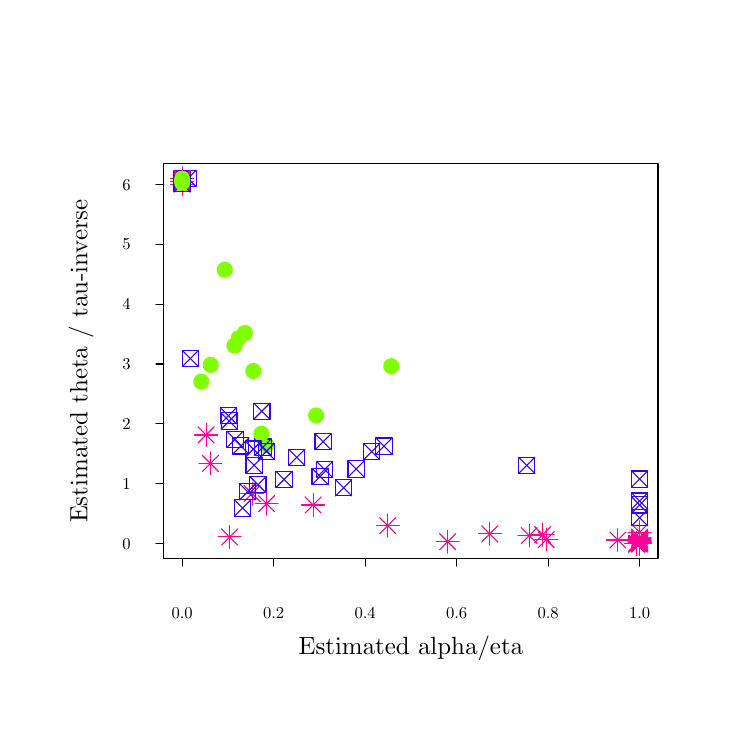
\begin{tikzpicture}[x=1pt,y=1pt]
\definecolor{fillColor}{RGB}{255,255,255}
\path[use as bounding box,fill=fillColor,fill opacity=0.00] (0,0) rectangle (252.94,252.94);
\begin{scope}
\path[clip] ( 49.20, 61.20) rectangle (227.75,203.75);
\definecolor{drawColor}{RGB}{255,0,153}

\path[draw=drawColor,line width= 0.4pt,line join=round,line cap=round] (218.21, 67.70) -- (224.06, 73.55);

\path[draw=drawColor,line width= 0.4pt,line join=round,line cap=round] (218.21, 73.55) -- (224.06, 67.70);

\path[draw=drawColor,line width= 0.4pt,line join=round,line cap=round] (216.99, 70.63) -- (225.27, 70.63);

\path[draw=drawColor,line width= 0.4pt,line join=round,line cap=round] (221.13, 66.49) -- (221.13, 74.77);

\path[draw=drawColor,line width= 0.4pt,line join=round,line cap=round] (218.21, 64.53) -- (224.06, 70.38);

\path[draw=drawColor,line width= 0.4pt,line join=round,line cap=round] (218.21, 70.38) -- (224.06, 64.53);

\path[draw=drawColor,line width= 0.4pt,line join=round,line cap=round] (217.00, 67.46) -- (225.27, 67.46);

\path[draw=drawColor,line width= 0.4pt,line join=round,line cap=round] (221.13, 63.32) -- (221.13, 71.59);

\path[draw=drawColor,line width= 0.4pt,line join=round,line cap=round] (217.14, 63.55) -- (222.99, 69.40);

\path[draw=drawColor,line width= 0.4pt,line join=round,line cap=round] (217.14, 69.40) -- (222.99, 63.55);

\path[draw=drawColor,line width= 0.4pt,line join=round,line cap=round] (215.93, 66.48) -- (224.21, 66.48);

\path[draw=drawColor,line width= 0.4pt,line join=round,line cap=round] (220.07, 62.34) -- (220.07, 70.62);
\definecolor{fillColor}{RGB}{128,255,0}

\path[fill=fillColor] ( 55.81,196.36) circle (  2.92);

\path[draw=drawColor,line width= 0.4pt,line join=round,line cap=round] ( 52.89,193.48) -- ( 58.74,199.33);

\path[draw=drawColor,line width= 0.4pt,line join=round,line cap=round] ( 52.89,199.33) -- ( 58.74,193.48);

\path[draw=drawColor,line width= 0.4pt,line join=round,line cap=round] ( 51.68,196.40) -- ( 59.95,196.40);

\path[draw=drawColor,line width= 0.4pt,line join=round,line cap=round] ( 55.81,192.27) -- ( 55.81,200.54);
\definecolor{drawColor}{RGB}{51,0,255}

\path[draw=drawColor,line width= 0.4pt,line join=round,line cap=round] (218.21, 78.96) rectangle (224.06, 84.81);

\path[draw=drawColor,line width= 0.4pt,line join=round,line cap=round] (218.21, 78.96) -- (224.06, 84.81);

\path[draw=drawColor,line width= 0.4pt,line join=round,line cap=round] (218.21, 84.81) -- (224.06, 78.96);

\path[fill=fillColor] ( 55.81,197.86) circle (  2.92);

\path[fill=fillColor] ( 55.81,197.47) circle (  2.92);

\path[fill=fillColor] ( 55.81,197.08) circle (  2.92);

\path[draw=drawColor,line width= 0.4pt,line join=round,line cap=round] ( 74.10, 98.87) rectangle ( 79.95,104.72);

\path[draw=drawColor,line width= 0.4pt,line join=round,line cap=round] ( 74.10, 98.87) -- ( 79.95,104.72);

\path[draw=drawColor,line width= 0.4pt,line join=round,line cap=round] ( 74.10,104.72) -- ( 79.95, 98.87);

\path[fill=fillColor] ( 78.50,142.61) circle (  2.92);

\path[draw=drawColor,line width= 0.4pt,line join=round,line cap=round] ( 52.89,195.14) rectangle ( 58.74,200.99);

\path[draw=drawColor,line width= 0.4pt,line join=round,line cap=round] ( 52.89,195.14) -- ( 58.74,200.99);

\path[draw=drawColor,line width= 0.4pt,line join=round,line cap=round] ( 52.89,200.99) -- ( 58.74,195.14);

\path[draw=drawColor,line width= 0.4pt,line join=round,line cap=round] (218.21, 86.91) rectangle (224.06, 92.76);

\path[draw=drawColor,line width= 0.4pt,line join=round,line cap=round] (218.21, 86.91) -- (224.06, 92.76);

\path[draw=drawColor,line width= 0.4pt,line join=round,line cap=round] (218.21, 92.76) -- (224.06, 86.91);
\definecolor{drawColor}{RGB}{255,0,153}

\path[draw=drawColor,line width= 0.4pt,line join=round,line cap=round] (184.42, 65.01) -- (190.27, 70.86);

\path[draw=drawColor,line width= 0.4pt,line join=round,line cap=round] (184.42, 70.86) -- (190.27, 65.01);

\path[draw=drawColor,line width= 0.4pt,line join=round,line cap=round] (183.21, 67.94) -- (191.49, 67.94);

\path[draw=drawColor,line width= 0.4pt,line join=round,line cap=round] (187.35, 63.80) -- (187.35, 72.07);
\definecolor{drawColor}{RGB}{51,0,255}

\path[draw=drawColor,line width= 0.4pt,line join=round,line cap=round] ( 81.70,111.44) rectangle ( 87.55,117.29);

\path[draw=drawColor,line width= 0.4pt,line join=round,line cap=round] ( 81.70,111.44) -- ( 87.55,117.29);

\path[draw=drawColor,line width= 0.4pt,line join=round,line cap=round] ( 81.70,117.29) -- ( 87.55,111.44);

\path[draw=drawColor,line width= 0.4pt,line join=round,line cap=round] (103.84,100.41) rectangle (109.69,106.26);

\path[draw=drawColor,line width= 0.4pt,line join=round,line cap=round] (103.84,100.41) -- (109.69,106.26);

\path[draw=drawColor,line width= 0.4pt,line join=round,line cap=round] (103.84,106.26) -- (109.69,100.41);

\path[draw=drawColor,line width= 0.4pt,line join=round,line cap=round] (104.36, 90.35) rectangle (110.21, 96.20);

\path[draw=drawColor,line width= 0.4pt,line join=round,line cap=round] (104.36, 90.35) -- (110.21, 96.20);

\path[draw=drawColor,line width= 0.4pt,line join=round,line cap=round] (104.36, 96.20) -- (110.21, 90.35);

\path[fill=fillColor] ( 55.81,196.52) circle (  2.92);

\path[fill=fillColor] ( 86.26,102.07) circle (  2.92);
\definecolor{drawColor}{RGB}{255,0,153}

\path[draw=drawColor,line width= 0.4pt,line join=round,line cap=round] (218.21, 64.28) -- (224.06, 70.13);

\path[draw=drawColor,line width= 0.4pt,line join=round,line cap=round] (218.21, 70.13) -- (224.06, 64.28);

\path[draw=drawColor,line width= 0.4pt,line join=round,line cap=round] (217.00, 67.20) -- (225.27, 67.20);

\path[draw=drawColor,line width= 0.4pt,line join=round,line cap=round] (221.13, 63.07) -- (221.13, 71.34);

\path[draw=drawColor,line width= 0.4pt,line join=round,line cap=round] (218.09, 63.55) -- (223.94, 69.40);

\path[draw=drawColor,line width= 0.4pt,line join=round,line cap=round] (218.09, 69.40) -- (223.94, 63.55);

\path[draw=drawColor,line width= 0.4pt,line join=round,line cap=round] (216.88, 66.48) -- (225.15, 66.48);

\path[draw=drawColor,line width= 0.4pt,line join=round,line cap=round] (221.01, 62.34) -- (221.01, 70.62);
\definecolor{drawColor}{RGB}{51,0,255}

\path[draw=drawColor,line width= 0.4pt,line join=round,line cap=round] ( 89.70, 86.76) rectangle ( 95.55, 92.61);

\path[draw=drawColor,line width= 0.4pt,line join=round,line cap=round] ( 89.70, 86.76) -- ( 95.55, 92.61);

\path[draw=drawColor,line width= 0.4pt,line join=round,line cap=round] ( 89.70, 92.61) -- ( 95.55, 86.76);
\definecolor{drawColor}{RGB}{255,0,153}

\path[draw=drawColor,line width= 0.4pt,line join=round,line cap=round] (148.84, 64.28) -- (154.69, 70.13);

\path[draw=drawColor,line width= 0.4pt,line join=round,line cap=round] (148.84, 70.13) -- (154.69, 64.28);

\path[draw=drawColor,line width= 0.4pt,line join=round,line cap=round] (147.63, 67.21) -- (155.90, 67.21);

\path[draw=drawColor,line width= 0.4pt,line join=round,line cap=round] (151.76, 63.07) -- (151.76, 71.34);

\path[draw=drawColor,line width= 0.4pt,line join=round,line cap=round] ( 52.89,194.35) -- ( 58.74,200.20);

\path[draw=drawColor,line width= 0.4pt,line join=round,line cap=round] ( 52.89,200.20) -- ( 58.74,194.35);

\path[draw=drawColor,line width= 0.4pt,line join=round,line cap=round] ( 51.68,197.28) -- ( 59.95,197.28);

\path[draw=drawColor,line width= 0.4pt,line join=round,line cap=round] ( 55.81,193.14) -- ( 55.81,201.41);

\path[draw=drawColor,line width= 0.4pt,line join=round,line cap=round] (218.09, 63.55) -- (223.94, 69.40);

\path[draw=drawColor,line width= 0.4pt,line join=round,line cap=round] (218.09, 69.40) -- (223.94, 63.55);

\path[draw=drawColor,line width= 0.4pt,line join=round,line cap=round] (216.88, 66.48) -- (225.15, 66.48);

\path[draw=drawColor,line width= 0.4pt,line join=round,line cap=round] (221.01, 62.34) -- (221.01, 70.62);

\path[fill=fillColor] (131.39,130.60) circle (  2.92);

\path[fill=fillColor] ( 62.76,125.04) circle (  2.92);

\path[draw=drawColor,line width= 0.4pt,line join=round,line cap=round] (217.14, 63.55) -- (222.99, 69.40);

\path[draw=drawColor,line width= 0.4pt,line join=round,line cap=round] (217.14, 69.40) -- (222.99, 63.55);

\path[draw=drawColor,line width= 0.4pt,line join=round,line cap=round] (215.93, 66.48) -- (224.21, 66.48);

\path[draw=drawColor,line width= 0.4pt,line join=round,line cap=round] (220.07, 62.34) -- (220.07, 70.62);

\path[draw=drawColor,line width= 0.4pt,line join=round,line cap=round] (100.20, 77.54) -- (106.05, 83.39);

\path[draw=drawColor,line width= 0.4pt,line join=round,line cap=round] (100.20, 83.39) -- (106.05, 77.54);

\path[draw=drawColor,line width= 0.4pt,line join=round,line cap=round] ( 98.99, 80.47) -- (107.27, 80.47);

\path[draw=drawColor,line width= 0.4pt,line join=round,line cap=round] (103.13, 76.33) -- (103.13, 84.60);
\definecolor{drawColor}{RGB}{51,0,255}

\path[draw=drawColor,line width= 0.4pt,line join=round,line cap=round] ( 83.30, 96.87) rectangle ( 89.15,102.72);

\path[draw=drawColor,line width= 0.4pt,line join=round,line cap=round] ( 83.30, 96.87) -- ( 89.15,102.72);

\path[draw=drawColor,line width= 0.4pt,line join=round,line cap=round] ( 83.30,102.72) -- ( 89.15, 96.87);
\definecolor{drawColor}{RGB}{255,0,153}

\path[draw=drawColor,line width= 0.4pt,line join=round,line cap=round] (218.09, 63.55) -- (223.94, 69.40);

\path[draw=drawColor,line width= 0.4pt,line join=round,line cap=round] (218.09, 69.40) -- (223.94, 63.55);

\path[draw=drawColor,line width= 0.4pt,line join=round,line cap=round] (216.88, 66.48) -- (225.15, 66.48);

\path[draw=drawColor,line width= 0.4pt,line join=round,line cap=round] (221.01, 62.34) -- (221.01, 70.62);
\definecolor{drawColor}{RGB}{51,0,255}

\path[draw=drawColor,line width= 0.4pt,line join=round,line cap=round] ( 94.31, 94.76) rectangle (100.16,100.61);

\path[draw=drawColor,line width= 0.4pt,line join=round,line cap=round] ( 94.31, 94.76) -- (100.16,100.61);

\path[draw=drawColor,line width= 0.4pt,line join=round,line cap=round] ( 94.31,100.61) -- (100.16, 94.76);

\path[draw=drawColor,line width= 0.4pt,line join=round,line cap=round] ( 69.59,109.77) rectangle ( 75.44,115.62);

\path[draw=drawColor,line width= 0.4pt,line join=round,line cap=round] ( 69.59,109.77) -- ( 75.44,115.62);

\path[draw=drawColor,line width= 0.4pt,line join=round,line cap=round] ( 69.59,115.62) -- ( 75.44,109.77);
\definecolor{drawColor}{RGB}{255,0,153}

\path[draw=drawColor,line width= 0.4pt,line join=round,line cap=round] ( 52.89,194.28) -- ( 58.74,200.13);

\path[draw=drawColor,line width= 0.4pt,line join=round,line cap=round] ( 52.89,200.13) -- ( 58.74,194.28);

\path[draw=drawColor,line width= 0.4pt,line join=round,line cap=round] ( 51.68,197.20) -- ( 59.95,197.20);

\path[draw=drawColor,line width= 0.4pt,line join=round,line cap=round] ( 55.81,193.07) -- ( 55.81,201.34);

\path[draw=drawColor,line width= 0.4pt,line join=round,line cap=round] (218.21, 63.55) -- (224.06, 69.40);

\path[draw=drawColor,line width= 0.4pt,line join=round,line cap=round] (218.21, 69.40) -- (224.06, 63.55);

\path[draw=drawColor,line width= 0.4pt,line join=round,line cap=round] (217.00, 66.48) -- (225.27, 66.48);

\path[draw=drawColor,line width= 0.4pt,line join=round,line cap=round] (221.13, 62.34) -- (221.13, 70.62);
\definecolor{drawColor}{RGB}{51,0,255}

\path[draw=drawColor,line width= 0.4pt,line join=round,line cap=round] ( 55.00,195.52) rectangle ( 60.85,201.37);

\path[draw=drawColor,line width= 0.4pt,line join=round,line cap=round] ( 55.00,195.52) -- ( 60.85,201.37);

\path[draw=drawColor,line width= 0.4pt,line join=round,line cap=round] ( 55.00,201.37) -- ( 60.85,195.52);

\path[draw=drawColor,line width= 0.4pt,line join=round,line cap=round] ( 82.10, 98.45) rectangle ( 87.95,104.30);

\path[draw=drawColor,line width= 0.4pt,line join=round,line cap=round] ( 82.10, 98.45) -- ( 87.95,104.30);

\path[draw=drawColor,line width= 0.4pt,line join=round,line cap=round] ( 82.10,104.30) -- ( 87.95, 98.45);

\path[fill=fillColor] ( 55.81,197.24) circle (  2.92);
\definecolor{drawColor}{RGB}{255,0,153}

\path[draw=drawColor,line width= 0.4pt,line join=round,line cap=round] ( 63.12, 92.55) -- ( 68.97, 98.40);

\path[draw=drawColor,line width= 0.4pt,line join=round,line cap=round] ( 63.12, 98.40) -- ( 68.97, 92.55);

\path[draw=drawColor,line width= 0.4pt,line join=round,line cap=round] ( 61.91, 95.47) -- ( 70.18, 95.47);

\path[draw=drawColor,line width= 0.4pt,line join=round,line cap=round] ( 66.04, 91.34) -- ( 66.04, 99.61);
\definecolor{drawColor}{RGB}{51,0,255}

\path[draw=drawColor,line width= 0.4pt,line join=round,line cap=round] (102.75, 87.84) rectangle (108.60, 93.69);

\path[draw=drawColor,line width= 0.4pt,line join=round,line cap=round] (102.75, 87.84) -- (108.60, 93.69);

\path[draw=drawColor,line width= 0.4pt,line join=round,line cap=round] (102.75, 93.69) -- (108.60, 87.84);

\path[fill=fillColor] ( 55.81,196.40) circle (  2.92);
\definecolor{drawColor}{RGB}{255,0,153}

\path[draw=drawColor,line width= 0.4pt,line join=round,line cap=round] (217.14, 63.55) -- (222.99, 69.40);

\path[draw=drawColor,line width= 0.4pt,line join=round,line cap=round] (217.14, 69.40) -- (222.99, 63.55);

\path[draw=drawColor,line width= 0.4pt,line join=round,line cap=round] (215.93, 66.48) -- (224.21, 66.48);

\path[draw=drawColor,line width= 0.4pt,line join=round,line cap=round] (220.07, 62.34) -- (220.07, 70.62);

\path[fill=fillColor] ( 76.29,140.79) circle (  2.92);

\path[draw=drawColor,line width= 0.4pt,line join=round,line cap=round] ( 61.54,102.85) -- ( 67.39,108.70);

\path[draw=drawColor,line width= 0.4pt,line join=round,line cap=round] ( 61.54,108.70) -- ( 67.39,102.85);

\path[draw=drawColor,line width= 0.4pt,line join=round,line cap=round] ( 60.33,105.77) -- ( 68.60,105.77);

\path[draw=drawColor,line width= 0.4pt,line join=round,line cap=round] ( 64.47,101.64) -- ( 64.47,109.91);

\path[draw=drawColor,line width= 0.4pt,line join=round,line cap=round] (217.14, 63.55) -- (222.99, 69.40);

\path[draw=drawColor,line width= 0.4pt,line join=round,line cap=round] (217.14, 69.40) -- (222.99, 63.55);

\path[draw=drawColor,line width= 0.4pt,line join=round,line cap=round] (215.93, 66.48) -- (224.21, 66.48);

\path[draw=drawColor,line width= 0.4pt,line join=round,line cap=round] (220.07, 62.34) -- (220.07, 70.62);
\definecolor{drawColor}{RGB}{51,0,255}

\path[draw=drawColor,line width= 0.4pt,line join=round,line cap=round] (111.26, 83.75) rectangle (117.11, 89.60);

\path[draw=drawColor,line width= 0.4pt,line join=round,line cap=round] (111.26, 83.75) -- (117.11, 89.60);

\path[draw=drawColor,line width= 0.4pt,line join=round,line cap=round] (111.26, 89.60) -- (117.11, 83.75);

\path[draw=drawColor,line width= 0.4pt,line join=round,line cap=round] ( 74.74, 76.46) rectangle ( 80.59, 82.31);

\path[draw=drawColor,line width= 0.4pt,line join=round,line cap=round] ( 74.74, 76.46) -- ( 80.59, 82.31);

\path[draw=drawColor,line width= 0.4pt,line join=round,line cap=round] ( 74.74, 82.31) -- ( 80.59, 76.46);

\path[fill=fillColor] ( 55.81,198.24) circle (  2.92);
\definecolor{drawColor}{RGB}{255,0,153}

\path[draw=drawColor,line width= 0.4pt,line join=round,line cap=round] (217.14, 63.55) -- (222.99, 69.40);

\path[draw=drawColor,line width= 0.4pt,line join=round,line cap=round] (217.14, 69.40) -- (222.99, 63.55);

\path[draw=drawColor,line width= 0.4pt,line join=round,line cap=round] (215.93, 66.48) -- (224.21, 66.48);

\path[draw=drawColor,line width= 0.4pt,line join=round,line cap=round] (220.07, 62.34) -- (220.07, 70.62);

\path[fill=fillColor] ( 55.81,197.55) circle (  2.92);

\path[fill=fillColor] ( 66.14,131.07) circle (  2.92);

\path[draw=drawColor,line width= 0.4pt,line join=round,line cap=round] ( 78.17, 81.66) -- ( 84.02, 87.51);

\path[draw=drawColor,line width= 0.4pt,line join=round,line cap=round] ( 78.17, 87.51) -- ( 84.02, 81.66);

\path[draw=drawColor,line width= 0.4pt,line join=round,line cap=round] ( 76.96, 84.59) -- ( 85.23, 84.59);

\path[draw=drawColor,line width= 0.4pt,line join=round,line cap=round] ( 81.10, 80.45) -- ( 81.10, 88.72);
\definecolor{drawColor}{RGB}{51,0,255}

\path[draw=drawColor,line width= 0.4pt,line join=round,line cap=round] ( 52.89,195.54) rectangle ( 58.74,201.39);

\path[draw=drawColor,line width= 0.4pt,line join=round,line cap=round] ( 52.89,195.54) -- ( 58.74,201.39);

\path[draw=drawColor,line width= 0.4pt,line join=round,line cap=round] ( 52.89,201.39) -- ( 58.74,195.54);
\definecolor{drawColor}{RGB}{255,0,153}

\path[draw=drawColor,line width= 0.4pt,line join=round,line cap=round] (178.32, 66.48) -- (184.17, 72.33);

\path[draw=drawColor,line width= 0.4pt,line join=round,line cap=round] (178.32, 72.33) -- (184.17, 66.48);

\path[draw=drawColor,line width= 0.4pt,line join=round,line cap=round] (177.11, 69.41) -- (185.38, 69.41);

\path[draw=drawColor,line width= 0.4pt,line join=round,line cap=round] (181.25, 65.27) -- (181.25, 73.54);

\path[fill=fillColor] ( 81.52,128.87) circle (  2.92);

\path[fill=fillColor] ( 71.21,165.47) circle (  2.92);

\path[draw=drawColor,line width= 0.4pt,line join=round,line cap=round] ( 52.89,194.34) -- ( 58.74,200.19);

\path[draw=drawColor,line width= 0.4pt,line join=round,line cap=round] ( 52.89,200.19) -- ( 58.74,194.34);

\path[draw=drawColor,line width= 0.4pt,line join=round,line cap=round] ( 51.68,197.27) -- ( 59.95,197.27);

\path[draw=drawColor,line width= 0.4pt,line join=round,line cap=round] ( 55.81,193.13) -- ( 55.81,201.40);

\path[draw=drawColor,line width= 0.4pt,line join=round,line cap=round] ( 52.89,195.48) -- ( 58.74,201.33);

\path[draw=drawColor,line width= 0.4pt,line join=round,line cap=round] ( 52.89,201.33) -- ( 58.74,195.48);

\path[draw=drawColor,line width= 0.4pt,line join=round,line cap=round] ( 51.68,198.41) -- ( 59.95,198.41);

\path[draw=drawColor,line width= 0.4pt,line join=round,line cap=round] ( 55.81,194.27) -- ( 55.81,202.55);
\definecolor{drawColor}{RGB}{51,0,255}

\path[draw=drawColor,line width= 0.4pt,line join=round,line cap=round] (218.21, 77.56) rectangle (224.06, 83.41);

\path[draw=drawColor,line width= 0.4pt,line join=round,line cap=round] (218.21, 77.56) -- (224.06, 83.41);

\path[draw=drawColor,line width= 0.4pt,line join=round,line cap=round] (218.21, 83.41) -- (224.06, 77.56);

\path[draw=drawColor,line width= 0.4pt,line join=round,line cap=round] ( 76.56, 82.29) rectangle ( 82.41, 88.14);

\path[draw=drawColor,line width= 0.4pt,line join=round,line cap=round] ( 76.56, 82.29) -- ( 82.41, 88.14);

\path[draw=drawColor,line width= 0.4pt,line join=round,line cap=round] ( 76.56, 88.14) -- ( 82.41, 82.29);
\definecolor{drawColor}{RGB}{255,0,153}

\path[draw=drawColor,line width= 0.4pt,line join=round,line cap=round] (218.21, 64.13) -- (224.06, 69.98);

\path[draw=drawColor,line width= 0.4pt,line join=round,line cap=round] (218.21, 69.98) -- (224.06, 64.13);

\path[draw=drawColor,line width= 0.4pt,line join=round,line cap=round] (217.00, 67.06) -- (225.27, 67.06);

\path[draw=drawColor,line width= 0.4pt,line join=round,line cap=round] (221.13, 62.92) -- (221.13, 71.19);
\definecolor{drawColor}{RGB}{51,0,255}

\path[draw=drawColor,line width= 0.4pt,line join=round,line cap=round] ( 71.99,101.26) rectangle ( 77.84,107.11);

\path[draw=drawColor,line width= 0.4pt,line join=round,line cap=round] ( 71.99,101.26) -- ( 77.84,107.11);

\path[draw=drawColor,line width= 0.4pt,line join=round,line cap=round] ( 71.99,107.11) -- ( 77.84,101.26);
\definecolor{drawColor}{RGB}{255,0,153}

\path[draw=drawColor,line width= 0.4pt,line join=round,line cap=round] (218.21, 63.55) -- (224.06, 69.40);

\path[draw=drawColor,line width= 0.4pt,line join=round,line cap=round] (218.21, 69.40) -- (224.06, 63.55);

\path[draw=drawColor,line width= 0.4pt,line join=round,line cap=round] (217.00, 66.48) -- (225.27, 66.48);

\path[draw=drawColor,line width= 0.4pt,line join=round,line cap=round] (221.13, 62.34) -- (221.13, 70.62);

\path[draw=drawColor,line width= 0.4pt,line join=round,line cap=round] ( 70.05, 65.99) -- ( 75.90, 71.84);

\path[draw=drawColor,line width= 0.4pt,line join=round,line cap=round] ( 70.05, 71.84) -- ( 75.90, 65.99);

\path[draw=drawColor,line width= 0.4pt,line join=round,line cap=round] ( 68.84, 68.92) -- ( 77.11, 68.92);

\path[draw=drawColor,line width= 0.4pt,line join=round,line cap=round] ( 72.98, 64.78) -- ( 72.98, 73.05);
\definecolor{drawColor}{RGB}{51,0,255}

\path[draw=drawColor,line width= 0.4pt,line join=round,line cap=round] ( 55.87,130.47) rectangle ( 61.72,136.32);

\path[draw=drawColor,line width= 0.4pt,line join=round,line cap=round] ( 55.87,130.47) -- ( 61.72,136.32);

\path[draw=drawColor,line width= 0.4pt,line join=round,line cap=round] ( 55.87,136.32) -- ( 61.72,130.47);
\definecolor{drawColor}{RGB}{255,0,153}

\path[draw=drawColor,line width= 0.4pt,line join=round,line cap=round] (218.21, 65.12) -- (224.06, 70.97);

\path[draw=drawColor,line width= 0.4pt,line join=round,line cap=round] (218.21, 70.97) -- (224.06, 65.12);

\path[draw=drawColor,line width= 0.4pt,line join=round,line cap=round] (217.00, 68.05) -- (225.27, 68.05);

\path[draw=drawColor,line width= 0.4pt,line join=round,line cap=round] (221.13, 63.91) -- (221.13, 72.18);

\path[draw=drawColor,line width= 0.4pt,line join=round,line cap=round] ( 52.89,195.42) -- ( 58.74,201.27);

\path[draw=drawColor,line width= 0.4pt,line join=round,line cap=round] ( 52.89,201.27) -- ( 58.74,195.42);

\path[draw=drawColor,line width= 0.4pt,line join=round,line cap=round] ( 51.68,198.35) -- ( 59.95,198.35);

\path[draw=drawColor,line width= 0.4pt,line join=round,line cap=round] ( 55.81,194.21) -- ( 55.81,202.48);

\path[fill=fillColor] ( 84.46,106.19) circle (  2.92);
\definecolor{drawColor}{RGB}{51,0,255}

\path[draw=drawColor,line width= 0.4pt,line join=round,line cap=round] ( 80.27, 84.89) rectangle ( 86.12, 90.74);

\path[draw=drawColor,line width= 0.4pt,line join=round,line cap=round] ( 80.27, 84.89) -- ( 86.12, 90.74);

\path[draw=drawColor,line width= 0.4pt,line join=round,line cap=round] ( 80.27, 90.74) -- ( 86.12, 84.89);
\definecolor{drawColor}{RGB}{255,0,153}

\path[draw=drawColor,line width= 0.4pt,line join=round,line cap=round] (127.20, 70.09) -- (133.05, 75.94);

\path[draw=drawColor,line width= 0.4pt,line join=round,line cap=round] (127.20, 75.94) -- (133.05, 70.09);

\path[draw=drawColor,line width= 0.4pt,line join=round,line cap=round] (125.99, 73.01) -- (134.26, 73.01);

\path[draw=drawColor,line width= 0.4pt,line join=round,line cap=round] (130.13, 68.88) -- (130.13, 77.15);

\path[draw=drawColor,line width= 0.4pt,line join=round,line cap=round] ( 83.40, 78.00) -- ( 89.25, 83.85);

\path[draw=drawColor,line width= 0.4pt,line join=round,line cap=round] ( 83.40, 83.85) -- ( 89.25, 78.00);

\path[draw=drawColor,line width= 0.4pt,line join=round,line cap=round] ( 82.18, 80.93) -- ( 90.46, 80.93);

\path[draw=drawColor,line width= 0.4pt,line join=round,line cap=round] ( 86.32, 76.79) -- ( 86.32, 85.06);

\path[draw=drawColor,line width= 0.4pt,line join=round,line cap=round] (217.14, 63.55) -- (222.99, 69.40);

\path[draw=drawColor,line width= 0.4pt,line join=round,line cap=round] (217.14, 69.40) -- (222.99, 63.55);

\path[draw=drawColor,line width= 0.4pt,line join=round,line cap=round] (215.93, 66.48) -- (224.21, 66.48);

\path[draw=drawColor,line width= 0.4pt,line join=round,line cap=round] (220.07, 62.34) -- (220.07, 70.62);

\path[draw=drawColor,line width= 0.4pt,line join=round,line cap=round] ( 52.89,195.45) -- ( 58.74,201.30);

\path[draw=drawColor,line width= 0.4pt,line join=round,line cap=round] ( 52.89,201.30) -- ( 58.74,195.45);

\path[draw=drawColor,line width= 0.4pt,line join=round,line cap=round] ( 51.68,198.37) -- ( 59.95,198.37);

\path[draw=drawColor,line width= 0.4pt,line join=round,line cap=round] ( 55.81,194.23) -- ( 55.81,202.51);

\path[draw=drawColor,line width= 0.4pt,line join=round,line cap=round] ( 52.89,194.59) -- ( 58.74,200.44);

\path[draw=drawColor,line width= 0.4pt,line join=round,line cap=round] ( 52.89,200.44) -- ( 58.74,194.59);

\path[draw=drawColor,line width= 0.4pt,line join=round,line cap=round] ( 51.68,197.51) -- ( 59.95,197.51);

\path[draw=drawColor,line width= 0.4pt,line join=round,line cap=round] ( 55.81,193.38) -- ( 55.81,201.65);
\definecolor{drawColor}{RGB}{51,0,255}

\path[draw=drawColor,line width= 0.4pt,line join=round,line cap=round] ( 78.91, 91.91) rectangle ( 84.76, 97.76);

\path[draw=drawColor,line width= 0.4pt,line join=round,line cap=round] ( 78.91, 91.91) -- ( 84.76, 97.76);

\path[draw=drawColor,line width= 0.4pt,line join=round,line cap=round] ( 78.91, 97.76) -- ( 84.76, 91.91);

\path[fill=fillColor] ( 55.81,198.37) circle (  2.92);

\path[draw=drawColor,line width= 0.4pt,line join=round,line cap=round] ( 52.89,193.73) rectangle ( 58.74,199.58);

\path[draw=drawColor,line width= 0.4pt,line join=round,line cap=round] ( 52.89,193.73) -- ( 58.74,199.58);

\path[draw=drawColor,line width= 0.4pt,line join=round,line cap=round] ( 52.89,199.58) -- ( 58.74,193.73);
\definecolor{drawColor}{RGB}{255,0,153}

\path[draw=drawColor,line width= 0.4pt,line join=round,line cap=round] (217.14, 63.55) -- (222.99, 69.40);

\path[draw=drawColor,line width= 0.4pt,line join=round,line cap=round] (217.14, 69.40) -- (222.99, 63.55);

\path[draw=drawColor,line width= 0.4pt,line join=round,line cap=round] (215.93, 66.48) -- (224.21, 66.48);

\path[draw=drawColor,line width= 0.4pt,line join=round,line cap=round] (220.07, 62.34) -- (220.07, 70.62);

\path[draw=drawColor,line width= 0.4pt,line join=round,line cap=round] (217.14, 63.55) -- (222.99, 69.40);

\path[draw=drawColor,line width= 0.4pt,line join=round,line cap=round] (217.14, 69.40) -- (222.99, 63.55);

\path[draw=drawColor,line width= 0.4pt,line join=round,line cap=round] (215.93, 66.48) -- (224.21, 66.48);

\path[draw=drawColor,line width= 0.4pt,line join=round,line cap=round] (220.07, 62.34) -- (220.07, 70.62);
\definecolor{drawColor}{RGB}{51,0,255}

\path[draw=drawColor,line width= 0.4pt,line join=round,line cap=round] (115.76, 90.55) rectangle (121.61, 96.40);

\path[draw=drawColor,line width= 0.4pt,line join=round,line cap=round] (115.76, 90.55) -- (121.61, 96.40);

\path[draw=drawColor,line width= 0.4pt,line join=round,line cap=round] (115.76, 96.40) -- (121.61, 90.55);

\path[fill=fillColor] ( 74.73,138.05) circle (  2.92);
\definecolor{drawColor}{RGB}{255,0,153}

\path[draw=drawColor,line width= 0.4pt,line join=round,line cap=round] (217.14, 63.55) -- (222.99, 69.40);

\path[draw=drawColor,line width= 0.4pt,line join=round,line cap=round] (217.14, 69.40) -- (222.99, 63.55);

\path[draw=drawColor,line width= 0.4pt,line join=round,line cap=round] (215.93, 66.48) -- (224.21, 66.48);

\path[draw=drawColor,line width= 0.4pt,line join=round,line cap=round] (220.07, 62.34) -- (220.07, 70.62);

\path[fill=fillColor] (104.23,112.82) circle (  2.92);

\path[draw=drawColor,line width= 0.4pt,line join=round,line cap=round] (218.21, 63.55) -- (224.06, 69.40);

\path[draw=drawColor,line width= 0.4pt,line join=round,line cap=round] (218.21, 69.40) -- (224.06, 63.55);

\path[draw=drawColor,line width= 0.4pt,line join=round,line cap=round] (217.00, 66.48) -- (225.27, 66.48);

\path[draw=drawColor,line width= 0.4pt,line join=round,line cap=round] (221.13, 62.34) -- (221.13, 70.62);

\path[draw=drawColor,line width= 0.4pt,line join=round,line cap=round] (217.14, 63.55) -- (222.99, 69.40);

\path[draw=drawColor,line width= 0.4pt,line join=round,line cap=round] (217.14, 69.40) -- (222.99, 63.55);

\path[draw=drawColor,line width= 0.4pt,line join=round,line cap=round] (215.93, 66.48) -- (224.21, 66.48);

\path[draw=drawColor,line width= 0.4pt,line join=round,line cap=round] (220.07, 62.34) -- (220.07, 70.62);
\definecolor{drawColor}{RGB}{51,0,255}

\path[draw=drawColor,line width= 0.4pt,line join=round,line cap=round] (121.40, 96.82) rectangle (127.25,102.67);

\path[draw=drawColor,line width= 0.4pt,line join=round,line cap=round] (121.40, 96.82) -- (127.25,102.67);

\path[draw=drawColor,line width= 0.4pt,line join=round,line cap=round] (121.40,102.67) -- (127.25, 96.82);
\definecolor{drawColor}{RGB}{255,0,153}

\path[draw=drawColor,line width= 0.4pt,line join=round,line cap=round] (218.21, 63.55) -- (224.06, 69.40);

\path[draw=drawColor,line width= 0.4pt,line join=round,line cap=round] (218.21, 69.40) -- (224.06, 63.55);

\path[draw=drawColor,line width= 0.4pt,line join=round,line cap=round] (217.00, 66.48) -- (225.27, 66.48);

\path[draw=drawColor,line width= 0.4pt,line join=round,line cap=round] (221.13, 62.34) -- (221.13, 70.62);

\path[fill=fillColor] ( 55.81,198.10) circle (  2.92);
\definecolor{drawColor}{RGB}{51,0,255}

\path[draw=drawColor,line width= 0.4pt,line join=round,line cap=round] ( 69.90,107.88) rectangle ( 75.75,113.73);

\path[draw=drawColor,line width= 0.4pt,line join=round,line cap=round] ( 69.90,107.88) -- ( 75.75,113.73);

\path[draw=drawColor,line width= 0.4pt,line join=round,line cap=round] ( 69.90,113.73) -- ( 75.75,107.88);
\definecolor{drawColor}{RGB}{255,0,153}

\path[draw=drawColor,line width= 0.4pt,line join=round,line cap=round] (217.14, 63.55) -- (222.99, 69.40);

\path[draw=drawColor,line width= 0.4pt,line join=round,line cap=round] (217.14, 69.40) -- (222.99, 63.55);

\path[draw=drawColor,line width= 0.4pt,line join=round,line cap=round] (215.93, 66.48) -- (224.21, 66.48);

\path[draw=drawColor,line width= 0.4pt,line join=round,line cap=round] (220.07, 62.34) -- (220.07, 70.62);

\path[draw=drawColor,line width= 0.4pt,line join=round,line cap=round] (164.06, 67.09) -- (169.91, 72.94);

\path[draw=drawColor,line width= 0.4pt,line join=round,line cap=round] (164.06, 72.94) -- (169.91, 67.09);

\path[draw=drawColor,line width= 0.4pt,line join=round,line cap=round] (162.85, 70.02) -- (171.12, 70.02);

\path[draw=drawColor,line width= 0.4pt,line join=round,line cap=round] (166.99, 65.88) -- (166.99, 74.15);
\definecolor{drawColor}{RGB}{51,0,255}

\path[draw=drawColor,line width= 0.4pt,line join=round,line cap=round] (125.84, 98.82) rectangle (131.69,104.67);

\path[draw=drawColor,line width= 0.4pt,line join=round,line cap=round] (125.84, 98.82) -- (131.69,104.67);

\path[draw=drawColor,line width= 0.4pt,line join=round,line cap=round] (125.84,104.67) -- (131.69, 98.82);

\path[draw=drawColor,line width= 0.4pt,line join=round,line cap=round] ( 78.63, 97.72) rectangle ( 84.48,103.57);

\path[draw=drawColor,line width= 0.4pt,line join=round,line cap=round] ( 78.63, 97.72) -- ( 84.48,103.57);

\path[draw=drawColor,line width= 0.4pt,line join=round,line cap=round] ( 78.63,103.57) -- ( 84.48, 97.72);
\definecolor{drawColor}{RGB}{255,0,153}

\path[draw=drawColor,line width= 0.4pt,line join=round,line cap=round] (218.21, 65.39) -- (224.06, 71.24);

\path[draw=drawColor,line width= 0.4pt,line join=round,line cap=round] (218.21, 71.24) -- (224.06, 65.39);

\path[draw=drawColor,line width= 0.4pt,line join=round,line cap=round] (217.00, 68.32) -- (225.27, 68.32);

\path[draw=drawColor,line width= 0.4pt,line join=round,line cap=round] (221.13, 64.18) -- (221.13, 72.46);

\path[draw=drawColor,line width= 0.4pt,line join=round,line cap=round] (217.14, 63.55) -- (222.99, 69.40);

\path[draw=drawColor,line width= 0.4pt,line join=round,line cap=round] (217.14, 69.40) -- (222.99, 63.55);

\path[draw=drawColor,line width= 0.4pt,line join=round,line cap=round] (215.93, 66.48) -- (224.21, 66.48);

\path[draw=drawColor,line width= 0.4pt,line join=round,line cap=round] (220.07, 62.34) -- (220.07, 70.62);
\definecolor{drawColor}{RGB}{51,0,255}

\path[draw=drawColor,line width= 0.4pt,line join=round,line cap=round] (218.21, 72.94) rectangle (224.06, 78.79);

\path[draw=drawColor,line width= 0.4pt,line join=round,line cap=round] (218.21, 72.94) -- (224.06, 78.79);

\path[draw=drawColor,line width= 0.4pt,line join=round,line cap=round] (218.21, 78.79) -- (224.06, 72.94);
\definecolor{drawColor}{RGB}{255,0,153}

\path[draw=drawColor,line width= 0.4pt,line join=round,line cap=round] (210.35, 64.88) -- (216.20, 70.73);

\path[draw=drawColor,line width= 0.4pt,line join=round,line cap=round] (210.35, 70.73) -- (216.20, 64.88);

\path[draw=drawColor,line width= 0.4pt,line join=round,line cap=round] (209.14, 67.81) -- (217.41, 67.81);

\path[draw=drawColor,line width= 0.4pt,line join=round,line cap=round] (213.27, 63.67) -- (213.27, 71.94);

\path[fill=fillColor] ( 55.81,197.65) circle (  2.92);

\path[draw=drawColor,line width= 0.4pt,line join=round,line cap=round] (218.20, 63.89) -- (224.05, 69.74);

\path[draw=drawColor,line width= 0.4pt,line join=round,line cap=round] (218.20, 69.74) -- (224.05, 63.89);

\path[draw=drawColor,line width= 0.4pt,line join=round,line cap=round] (216.99, 66.82) -- (225.26, 66.82);

\path[draw=drawColor,line width= 0.4pt,line join=round,line cap=round] (221.13, 62.68) -- (221.13, 70.95);

\path[draw=drawColor,line width= 0.4pt,line join=round,line cap=round] (217.14, 63.55) -- (222.99, 69.40);

\path[draw=drawColor,line width= 0.4pt,line join=round,line cap=round] (217.14, 69.40) -- (222.99, 63.55);

\path[draw=drawColor,line width= 0.4pt,line join=round,line cap=round] (215.93, 66.48) -- (224.21, 66.48);

\path[draw=drawColor,line width= 0.4pt,line join=round,line cap=round] (220.07, 62.34) -- (220.07, 70.62);

\path[draw=drawColor,line width= 0.4pt,line join=round,line cap=round] (218.21, 65.90) -- (224.06, 71.75);

\path[draw=drawColor,line width= 0.4pt,line join=round,line cap=round] (218.21, 71.75) -- (224.06, 65.90);

\path[draw=drawColor,line width= 0.4pt,line join=round,line cap=round] (217.00, 68.83) -- (225.27, 68.83);

\path[draw=drawColor,line width= 0.4pt,line join=round,line cap=round] (221.13, 64.69) -- (221.13, 72.97);

\path[draw=drawColor,line width= 0.4pt,line join=round,line cap=round] (183.17, 66.80) -- (189.02, 72.65);

\path[draw=drawColor,line width= 0.4pt,line join=round,line cap=round] (183.17, 72.65) -- (189.02, 66.80);

\path[draw=drawColor,line width= 0.4pt,line join=round,line cap=round] (181.96, 69.72) -- (190.23, 69.72);

\path[draw=drawColor,line width= 0.4pt,line join=round,line cap=round] (186.10, 65.59) -- (186.10, 73.86);

\path[fill=fillColor] ( 55.81,197.02) circle (  2.92);
\definecolor{drawColor}{RGB}{51,0,255}

\path[draw=drawColor,line width= 0.4pt,line join=round,line cap=round] (177.43, 91.84) rectangle (183.28, 97.69);

\path[draw=drawColor,line width= 0.4pt,line join=round,line cap=round] (177.43, 91.84) -- (183.28, 97.69);

\path[draw=drawColor,line width= 0.4pt,line join=round,line cap=round] (177.43, 97.69) -- (183.28, 91.84);
\end{scope}
\begin{scope}
\path[clip] (  0.00,  0.00) rectangle (252.94,252.94);
\definecolor{drawColor}{RGB}{0,0,0}

\path[draw=drawColor,line width= 0.4pt,line join=round,line cap=round] ( 55.81, 61.20) -- (221.13, 61.20);

\path[draw=drawColor,line width= 0.4pt,line join=round,line cap=round] ( 55.81, 61.20) -- ( 55.81, 58.35);

\path[draw=drawColor,line width= 0.4pt,line join=round,line cap=round] ( 88.88, 61.20) -- ( 88.88, 58.35);

\path[draw=drawColor,line width= 0.4pt,line join=round,line cap=round] (121.94, 61.20) -- (121.94, 58.35);

\path[draw=drawColor,line width= 0.4pt,line join=round,line cap=round] (155.00, 61.20) -- (155.00, 58.35);

\path[draw=drawColor,line width= 0.4pt,line join=round,line cap=round] (188.07, 61.20) -- (188.07, 58.35);

\path[draw=drawColor,line width= 0.4pt,line join=round,line cap=round] (221.13, 61.20) -- (221.13, 58.35);

\node[text=drawColor,anchor=base,inner sep=0pt, outer sep=0pt, scale=  0.60] at ( 55.81, 39.60) {0.0};

\node[text=drawColor,anchor=base,inner sep=0pt, outer sep=0pt, scale=  0.60] at ( 88.88, 39.60) {0.2};

\node[text=drawColor,anchor=base,inner sep=0pt, outer sep=0pt, scale=  0.60] at (121.94, 39.60) {0.4};

\node[text=drawColor,anchor=base,inner sep=0pt, outer sep=0pt, scale=  0.60] at (155.00, 39.60) {0.6};

\node[text=drawColor,anchor=base,inner sep=0pt, outer sep=0pt, scale=  0.60] at (188.07, 39.60) {0.8};

\node[text=drawColor,anchor=base,inner sep=0pt, outer sep=0pt, scale=  0.60] at (221.13, 39.60) {1.0};

\path[draw=drawColor,line width= 0.4pt,line join=round,line cap=round] ( 49.20, 66.48) -- ( 49.20,196.32);

\path[draw=drawColor,line width= 0.4pt,line join=round,line cap=round] ( 49.20, 66.48) -- ( 46.35, 66.48);

\path[draw=drawColor,line width= 0.4pt,line join=round,line cap=round] ( 49.20, 88.12) -- ( 46.35, 88.12);

\path[draw=drawColor,line width= 0.4pt,line join=round,line cap=round] ( 49.20,109.76) -- ( 46.35,109.76);

\path[draw=drawColor,line width= 0.4pt,line join=round,line cap=round] ( 49.20,131.40) -- ( 46.35,131.40);

\path[draw=drawColor,line width= 0.4pt,line join=round,line cap=round] ( 49.20,153.04) -- ( 46.35,153.04);

\path[draw=drawColor,line width= 0.4pt,line join=round,line cap=round] ( 49.20,174.68) -- ( 46.35,174.68);

\path[draw=drawColor,line width= 0.4pt,line join=round,line cap=round] ( 49.20,196.32) -- ( 46.35,196.32);

\node[text=drawColor,anchor=base east,inner sep=0pt, outer sep=0pt, scale=  0.60] at ( 37.20, 64.41) {0};

\node[text=drawColor,anchor=base east,inner sep=0pt, outer sep=0pt, scale=  0.60] at ( 37.20, 86.05) {1};

\node[text=drawColor,anchor=base east,inner sep=0pt, outer sep=0pt, scale=  0.60] at ( 37.20,107.69) {2};

\node[text=drawColor,anchor=base east,inner sep=0pt, outer sep=0pt, scale=  0.60] at ( 37.20,129.33) {3};

\node[text=drawColor,anchor=base east,inner sep=0pt, outer sep=0pt, scale=  0.60] at ( 37.20,150.97) {4};

\node[text=drawColor,anchor=base east,inner sep=0pt, outer sep=0pt, scale=  0.60] at ( 37.20,172.61) {5};

\node[text=drawColor,anchor=base east,inner sep=0pt, outer sep=0pt, scale=  0.60] at ( 37.20,194.25) {6};

\path[draw=drawColor,line width= 0.4pt,line join=round,line cap=round] ( 49.20, 61.20) --
	(227.75, 61.20) --
	(227.75,203.75) --
	( 49.20,203.75) --
	( 49.20, 61.20);
\end{scope}
\begin{scope}
\path[clip] (  0.00,  0.00) rectangle (252.94,252.94);
\definecolor{drawColor}{RGB}{0,0,0}

\node[text=drawColor,anchor=base,inner sep=0pt, outer sep=0pt, scale=  0.90] at (138.47, 26.40) {Estimated alpha/eta};

\node[text=drawColor,rotate= 90.00,anchor=base,inner sep=0pt, outer sep=0pt, scale=  0.90] at ( 21.60,132.47) {Estimated theta / tau-inverse};
\end{scope}
\end{tikzpicture}

\end{frame}

\begin{frame}{Experiment Results}
	\framesubtitle{Multi arm bandit experiments - 2 Clusters / Spectral RBF / Blockwise Entropy}
	\center
	% Created by tikzDevice version 0.10.1 on 2016-06-29 14:24:24
% !TEX encoding = UTF-8 Unicode
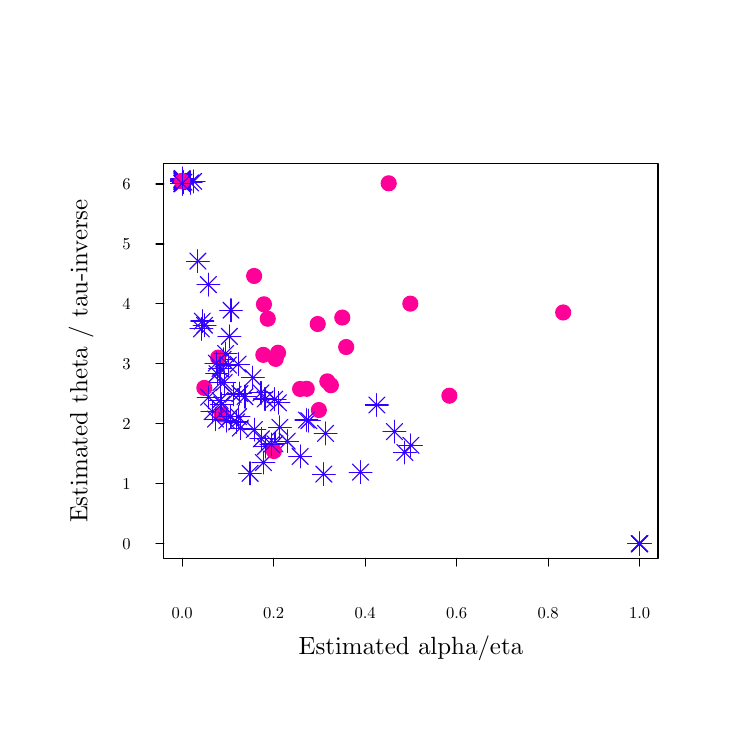
\begin{tikzpicture}[x=1pt,y=1pt]
\definecolor{fillColor}{RGB}{255,255,255}
\path[use as bounding box,fill=fillColor,fill opacity=0.00] (0,0) rectangle (252.94,252.94);
\begin{scope}
\path[clip] ( 49.20, 61.20) rectangle (227.75,203.75);
\definecolor{drawColor}{RGB}{51,0,255}

\path[draw=drawColor,line width= 0.4pt,line join=round,line cap=round] ( 62.35,157.19) -- ( 68.20,163.04);

\path[draw=drawColor,line width= 0.4pt,line join=round,line cap=round] ( 62.35,163.04) -- ( 68.20,157.19);

\path[draw=drawColor,line width= 0.4pt,line join=round,line cap=round] ( 61.14,160.12) -- ( 69.41,160.12);

\path[draw=drawColor,line width= 0.4pt,line join=round,line cap=round] ( 65.27,155.98) -- ( 65.27,164.25);

\path[draw=drawColor,line width= 0.4pt,line join=round,line cap=round] ( 67.72,130.20) -- ( 73.57,136.05);

\path[draw=drawColor,line width= 0.4pt,line join=round,line cap=round] ( 67.72,136.05) -- ( 73.57,130.20);

\path[draw=drawColor,line width= 0.4pt,line join=round,line cap=round] ( 66.51,133.12) -- ( 74.79,133.12);

\path[draw=drawColor,line width= 0.4pt,line join=round,line cap=round] ( 70.65,128.99) -- ( 70.65,137.26);

\path[draw=drawColor,line width= 0.4pt,line join=round,line cap=round] (218.21, 63.55) -- (224.06, 69.40);

\path[draw=drawColor,line width= 0.4pt,line join=round,line cap=round] (218.21, 69.40) -- (224.06, 63.55);

\path[draw=drawColor,line width= 0.4pt,line join=round,line cap=round] (217.00, 66.48) -- (225.27, 66.48);

\path[draw=drawColor,line width= 0.4pt,line join=round,line cap=round] (221.13, 62.34) -- (221.13, 70.62);
\definecolor{fillColor}{RGB}{255,0,153}

\path[fill=fillColor] (109.56,123.73) circle (  2.92);

\path[draw=drawColor,line width= 0.4pt,line join=round,line cap=round] ( 81.38,118.06) -- ( 87.23,123.91);

\path[draw=drawColor,line width= 0.4pt,line join=round,line cap=round] ( 81.38,123.91) -- ( 87.23,118.06);

\path[draw=drawColor,line width= 0.4pt,line join=round,line cap=round] ( 80.17,120.99) -- ( 88.44,120.99);

\path[draw=drawColor,line width= 0.4pt,line join=round,line cap=round] ( 84.30,116.85) -- ( 84.30,125.12);

\path[fill=fillColor] ( 63.83,122.76) circle (  2.92);

\path[draw=drawColor,line width= 0.4pt,line join=round,line cap=round] ( 86.43, 99.65) -- ( 92.28,105.50);

\path[draw=drawColor,line width= 0.4pt,line join=round,line cap=round] ( 86.43,105.50) -- ( 92.28, 99.65);

\path[draw=drawColor,line width= 0.4pt,line join=round,line cap=round] ( 85.22,102.57) -- ( 93.49,102.57);

\path[draw=drawColor,line width= 0.4pt,line join=round,line cap=round] ( 89.36, 98.44) -- ( 89.36,106.71);

\path[fill=fillColor] (130.46,196.70) circle (  2.92);

\path[draw=drawColor,line width= 0.4pt,line join=round,line cap=round] ( 87.66,114.47) -- ( 93.51,120.32);

\path[draw=drawColor,line width= 0.4pt,line join=round,line cap=round] ( 87.66,120.32) -- ( 93.51,114.47);

\path[draw=drawColor,line width= 0.4pt,line join=round,line cap=round] ( 86.45,117.40) -- ( 94.72,117.40);

\path[draw=drawColor,line width= 0.4pt,line join=round,line cap=round] ( 90.59,113.26) -- ( 90.59,121.53);

\path[fill=fillColor] ( 68.83,133.69) circle (  2.92);

\path[draw=drawColor,line width= 0.4pt,line join=round,line cap=round] ( 52.89,194.48) -- ( 58.74,200.33);

\path[draw=drawColor,line width= 0.4pt,line join=round,line cap=round] ( 52.89,200.33) -- ( 58.74,194.48);

\path[draw=drawColor,line width= 0.4pt,line join=round,line cap=round] ( 51.68,197.41) -- ( 59.95,197.41);

\path[draw=drawColor,line width= 0.4pt,line join=round,line cap=round] ( 55.81,193.27) -- ( 55.81,201.54);

\path[draw=drawColor,line width= 0.4pt,line join=round,line cap=round] ( 81.54,101.44) -- ( 87.39,107.29);

\path[draw=drawColor,line width= 0.4pt,line join=round,line cap=round] ( 81.54,107.29) -- ( 87.39,101.44);

\path[draw=drawColor,line width= 0.4pt,line join=round,line cap=round] ( 80.33,104.36) -- ( 88.60,104.36);

\path[draw=drawColor,line width= 0.4pt,line join=round,line cap=round] ( 84.47,100.23) -- ( 84.47,108.50);

\path[draw=drawColor,line width= 0.4pt,line join=round,line cap=round] ( 53.52,194.19) -- ( 59.37,200.04);

\path[draw=drawColor,line width= 0.4pt,line join=round,line cap=round] ( 53.52,200.04) -- ( 59.37,194.19);

\path[draw=drawColor,line width= 0.4pt,line join=round,line cap=round] ( 52.31,197.12) -- ( 60.59,197.12);

\path[draw=drawColor,line width= 0.4pt,line join=round,line cap=round] ( 56.45,192.98) -- ( 56.45,201.25);

\path[draw=drawColor,line width= 0.4pt,line join=round,line cap=round] ( 71.31,117.52) -- ( 77.16,123.37);

\path[draw=drawColor,line width= 0.4pt,line join=round,line cap=round] ( 71.31,123.37) -- ( 77.16,117.52);

\path[draw=drawColor,line width= 0.4pt,line join=round,line cap=round] ( 70.09,120.45) -- ( 78.37,120.45);

\path[draw=drawColor,line width= 0.4pt,line join=round,line cap=round] ( 74.23,116.31) -- ( 74.23,124.58);

\path[draw=drawColor,line width= 0.4pt,line join=round,line cap=round] ( 52.89,194.63) -- ( 58.74,200.48);

\path[draw=drawColor,line width= 0.4pt,line join=round,line cap=round] ( 52.89,200.48) -- ( 58.74,194.63);

\path[draw=drawColor,line width= 0.4pt,line join=round,line cap=round] ( 51.68,197.56) -- ( 59.95,197.56);

\path[draw=drawColor,line width= 0.4pt,line join=round,line cap=round] ( 55.81,193.42) -- ( 55.81,201.69);

\path[draw=drawColor,line width= 0.4pt,line join=round,line cap=round] ( 52.89,194.60) -- ( 58.74,200.45);

\path[draw=drawColor,line width= 0.4pt,line join=round,line cap=round] ( 52.89,200.45) -- ( 58.74,194.60);

\path[draw=drawColor,line width= 0.4pt,line join=round,line cap=round] ( 51.68,197.52) -- ( 59.95,197.52);

\path[draw=drawColor,line width= 0.4pt,line join=round,line cap=round] ( 55.81,193.39) -- ( 55.81,201.66);

\path[fill=fillColor] (104.82,145.86) circle (  2.92);

\path[draw=drawColor,line width= 0.4pt,line join=round,line cap=round] ( 62.47,116.50) -- ( 68.32,122.35);

\path[draw=drawColor,line width= 0.4pt,line join=round,line cap=round] ( 62.47,122.35) -- ( 68.32,116.50);

\path[draw=drawColor,line width= 0.4pt,line join=round,line cap=round] ( 61.26,119.43) -- ( 69.53,119.43);

\path[draw=drawColor,line width= 0.4pt,line join=round,line cap=round] ( 65.40,115.29) -- ( 65.40,123.56);

\path[draw=drawColor,line width= 0.4pt,line join=round,line cap=round] ( 98.67,108.01) -- (104.52,113.86);

\path[draw=drawColor,line width= 0.4pt,line join=round,line cap=round] ( 98.67,113.86) -- (104.52,108.01);

\path[draw=drawColor,line width= 0.4pt,line join=round,line cap=round] ( 97.45,110.93) -- (105.73,110.93);

\path[draw=drawColor,line width= 0.4pt,line join=round,line cap=round] (101.59,106.80) -- (101.59,115.07);

\path[draw=drawColor,line width= 0.4pt,line join=round,line cap=round] ( 52.89,193.75) -- ( 58.74,199.60);

\path[draw=drawColor,line width= 0.4pt,line join=round,line cap=round] ( 52.89,199.60) -- ( 58.74,193.75);

\path[draw=drawColor,line width= 0.4pt,line join=round,line cap=round] ( 51.68,196.68) -- ( 59.95,196.68);

\path[draw=drawColor,line width= 0.4pt,line join=round,line cap=round] ( 55.81,192.54) -- ( 55.81,200.81);

\path[draw=drawColor,line width= 0.4pt,line join=round,line cap=round] (218.09, 63.55) -- (223.94, 69.40);

\path[draw=drawColor,line width= 0.4pt,line join=round,line cap=round] (218.09, 69.40) -- (223.94, 63.55);

\path[draw=drawColor,line width= 0.4pt,line join=round,line cap=round] (216.88, 66.48) -- (225.15, 66.48);

\path[draw=drawColor,line width= 0.4pt,line join=round,line cap=round] (221.01, 62.34) -- (221.01, 70.62);

\path[draw=drawColor,line width= 0.4pt,line join=round,line cap=round] ( 73.76,117.78) -- ( 79.61,123.63);

\path[draw=drawColor,line width= 0.4pt,line join=round,line cap=round] ( 73.76,123.63) -- ( 79.61,117.78);

\path[draw=drawColor,line width= 0.4pt,line join=round,line cap=round] ( 72.54,120.70) -- ( 80.82,120.70);

\path[draw=drawColor,line width= 0.4pt,line join=round,line cap=round] ( 76.68,116.57) -- ( 76.68,124.84);

\path[draw=drawColor,line width= 0.4pt,line join=round,line cap=round] ( 66.57,126.82) -- ( 72.42,132.67);

\path[draw=drawColor,line width= 0.4pt,line join=round,line cap=round] ( 66.57,132.67) -- ( 72.42,126.82);

\path[draw=drawColor,line width= 0.4pt,line join=round,line cap=round] ( 65.36,129.74) -- ( 73.63,129.74);

\path[draw=drawColor,line width= 0.4pt,line join=round,line cap=round] ( 69.50,125.61) -- ( 69.50,133.88);

\path[draw=drawColor,line width= 0.4pt,line join=round,line cap=round] ( 52.89,195.54) -- ( 58.74,201.39);

\path[draw=drawColor,line width= 0.4pt,line join=round,line cap=round] ( 52.89,201.39) -- ( 58.74,195.54);

\path[draw=drawColor,line width= 0.4pt,line join=round,line cap=round] ( 51.68,198.47) -- ( 59.95,198.47);

\path[draw=drawColor,line width= 0.4pt,line join=round,line cap=round] ( 55.81,194.33) -- ( 55.81,202.60);

\path[draw=drawColor,line width= 0.4pt,line join=round,line cap=round] ( 63.79,111.31) -- ( 69.64,117.16);

\path[draw=drawColor,line width= 0.4pt,line join=round,line cap=round] ( 63.79,117.16) -- ( 69.64,111.31);

\path[draw=drawColor,line width= 0.4pt,line join=round,line cap=round] ( 62.57,114.23) -- ( 70.85,114.23);

\path[draw=drawColor,line width= 0.4pt,line join=round,line cap=round] ( 66.71,110.10) -- ( 66.71,118.37);

\path[fill=fillColor] ( 55.81,197.59) circle (  2.92);

\path[draw=drawColor,line width= 0.4pt,line join=round,line cap=round] ( 58.59,165.67) -- ( 64.44,171.52);

\path[draw=drawColor,line width= 0.4pt,line join=round,line cap=round] ( 58.59,171.52) -- ( 64.44,165.67);

\path[draw=drawColor,line width= 0.4pt,line join=round,line cap=round] ( 57.38,168.59) -- ( 65.66,168.59);

\path[draw=drawColor,line width= 0.4pt,line join=round,line cap=round] ( 61.52,164.45) -- ( 61.52,172.73);

\path[draw=drawColor,line width= 0.4pt,line join=round,line cap=round] (218.21, 63.55) -- (224.06, 69.40);

\path[draw=drawColor,line width= 0.4pt,line join=round,line cap=round] (218.21, 69.40) -- (224.06, 63.55);

\path[draw=drawColor,line width= 0.4pt,line join=round,line cap=round] (217.00, 66.48) -- (225.27, 66.48);

\path[draw=drawColor,line width= 0.4pt,line join=round,line cap=round] (221.13, 62.34) -- (221.13, 70.62);

\path[draw=drawColor,line width= 0.4pt,line join=round,line cap=round] ( 60.98,142.48) -- ( 66.83,148.33);

\path[draw=drawColor,line width= 0.4pt,line join=round,line cap=round] ( 60.98,148.33) -- ( 66.83,142.48);

\path[draw=drawColor,line width= 0.4pt,line join=round,line cap=round] ( 59.77,145.41) -- ( 68.04,145.41);

\path[draw=drawColor,line width= 0.4pt,line join=round,line cap=round] ( 63.90,141.27) -- ( 63.90,149.55);

\path[draw=drawColor,line width= 0.4pt,line join=round,line cap=round] ( 86.33,115.77) -- ( 92.18,121.62);

\path[draw=drawColor,line width= 0.4pt,line join=round,line cap=round] ( 86.33,121.62) -- ( 92.18,115.77);

\path[draw=drawColor,line width= 0.4pt,line join=round,line cap=round] ( 85.12,118.70) -- ( 93.39,118.70);

\path[draw=drawColor,line width= 0.4pt,line join=round,line cap=round] ( 89.26,114.56) -- ( 89.26,122.83);

\path[draw=drawColor,line width= 0.4pt,line join=round,line cap=round] ( 78.46,123.54) -- ( 84.31,129.39);

\path[draw=drawColor,line width= 0.4pt,line join=round,line cap=round] ( 78.46,129.39) -- ( 84.31,123.54);

\path[draw=drawColor,line width= 0.4pt,line join=round,line cap=round] ( 77.24,126.46) -- ( 85.52,126.46);

\path[draw=drawColor,line width= 0.4pt,line join=round,line cap=round] ( 81.38,122.33) -- ( 81.38,130.60);

\path[draw=drawColor,line width= 0.4pt,line join=round,line cap=round] ( 72.59,107.54) -- ( 78.44,113.39);

\path[draw=drawColor,line width= 0.4pt,line join=round,line cap=round] ( 72.59,113.39) -- ( 78.44,107.54);

\path[draw=drawColor,line width= 0.4pt,line join=round,line cap=round] ( 71.38,110.46) -- ( 79.65,110.46);

\path[draw=drawColor,line width= 0.4pt,line join=round,line cap=round] ( 75.51,106.33) -- ( 75.51,114.60);

\path[draw=drawColor,line width= 0.4pt,line join=round,line cap=round] ( 82.96, 98.61) -- ( 88.81,104.46);

\path[draw=drawColor,line width= 0.4pt,line join=round,line cap=round] ( 82.96,104.46) -- ( 88.81, 98.61);

\path[draw=drawColor,line width= 0.4pt,line join=round,line cap=round] ( 81.75,101.53) -- ( 90.02,101.53);

\path[draw=drawColor,line width= 0.4pt,line join=round,line cap=round] ( 85.88, 97.39) -- ( 85.88,105.67);

\path[draw=drawColor,line width= 0.4pt,line join=round,line cap=round] ( 69.96,138.46) -- ( 75.81,144.31);

\path[draw=drawColor,line width= 0.4pt,line join=round,line cap=round] ( 69.96,144.31) -- ( 75.81,138.46);

\path[draw=drawColor,line width= 0.4pt,line join=round,line cap=round] ( 68.75,141.38) -- ( 77.03,141.38);

\path[draw=drawColor,line width= 0.4pt,line join=round,line cap=round] ( 72.89,137.24) -- ( 72.89,145.52);

\path[draw=drawColor,line width= 0.4pt,line join=round,line cap=round] (104.09, 88.70) -- (109.94, 94.55);

\path[draw=drawColor,line width= 0.4pt,line join=round,line cap=round] (104.09, 94.55) -- (109.94, 88.70);

\path[draw=drawColor,line width= 0.4pt,line join=round,line cap=round] (102.88, 91.62) -- (111.15, 91.62);

\path[draw=drawColor,line width= 0.4pt,line join=round,line cap=round] (107.02, 87.48) -- (107.02, 95.76);

\path[draw=drawColor,line width= 0.4pt,line join=round,line cap=round] (218.21, 63.55) -- (224.06, 69.40);

\path[draw=drawColor,line width= 0.4pt,line join=round,line cap=round] (218.21, 69.40) -- (224.06, 63.55);

\path[draw=drawColor,line width= 0.4pt,line join=round,line cap=round] (217.00, 66.48) -- (225.27, 66.48);

\path[draw=drawColor,line width= 0.4pt,line join=round,line cap=round] (221.13, 62.34) -- (221.13, 70.62);

\path[fill=fillColor] (105.22,114.77) circle (  2.92);

\path[draw=drawColor,line width= 0.4pt,line join=round,line cap=round] ( 52.89,195.12) -- ( 58.74,200.97);

\path[draw=drawColor,line width= 0.4pt,line join=round,line cap=round] ( 52.89,200.97) -- ( 58.74,195.12);

\path[draw=drawColor,line width= 0.4pt,line join=round,line cap=round] ( 51.68,198.04) -- ( 59.95,198.04);

\path[draw=drawColor,line width= 0.4pt,line join=round,line cap=round] ( 55.81,193.90) -- ( 55.81,202.18);

\path[draw=drawColor,line width= 0.4pt,line join=round,line cap=round] (117.35, 89.42) -- (123.20, 95.27);

\path[draw=drawColor,line width= 0.4pt,line join=round,line cap=round] (117.35, 95.27) -- (123.20, 89.42);

\path[draw=drawColor,line width= 0.4pt,line join=round,line cap=round] (116.13, 92.35) -- (124.41, 92.35);

\path[draw=drawColor,line width= 0.4pt,line join=round,line cap=round] (120.27, 88.21) -- (120.27, 96.48);

\path[draw=drawColor,line width= 0.4pt,line join=round,line cap=round] (133.40, 96.50) -- (139.25,102.35);

\path[draw=drawColor,line width= 0.4pt,line join=round,line cap=round] (133.40,102.35) -- (139.25, 96.50);

\path[draw=drawColor,line width= 0.4pt,line join=round,line cap=round] (132.18, 99.42) -- (140.46, 99.42);

\path[draw=drawColor,line width= 0.4pt,line join=round,line cap=round] (136.32, 95.29) -- (136.32,103.56);

\path[draw=drawColor,line width= 0.4pt,line join=round,line cap=round] ( 68.06,121.82) -- ( 73.91,127.67);

\path[draw=drawColor,line width= 0.4pt,line join=round,line cap=round] ( 68.06,127.67) -- ( 73.91,121.82);

\path[draw=drawColor,line width= 0.4pt,line join=round,line cap=round] ( 66.85,124.75) -- ( 75.12,124.75);

\path[draw=drawColor,line width= 0.4pt,line join=round,line cap=round] ( 70.98,120.61) -- ( 70.98,128.89);

\path[draw=drawColor,line width= 0.4pt,line join=round,line cap=round] ( 69.59,128.11) -- ( 75.44,133.96);

\path[draw=drawColor,line width= 0.4pt,line join=round,line cap=round] ( 69.59,133.96) -- ( 75.44,128.11);

\path[draw=drawColor,line width= 0.4pt,line join=round,line cap=round] ( 68.38,131.03) -- ( 76.65,131.03);

\path[draw=drawColor,line width= 0.4pt,line join=round,line cap=round] ( 72.52,126.89) -- ( 72.52,135.17);

\path[draw=drawColor,line width= 0.4pt,line join=round,line cap=round] ( 52.89,194.32) -- ( 58.74,200.17);

\path[draw=drawColor,line width= 0.4pt,line join=round,line cap=round] ( 52.89,200.17) -- ( 58.74,194.32);

\path[draw=drawColor,line width= 0.4pt,line join=round,line cap=round] ( 51.68,197.25) -- ( 59.95,197.25);

\path[draw=drawColor,line width= 0.4pt,line join=round,line cap=round] ( 55.81,193.11) -- ( 55.81,201.38);

\path[draw=drawColor,line width= 0.4pt,line join=round,line cap=round] ( 52.89,195.15) -- ( 58.74,201.00);

\path[draw=drawColor,line width= 0.4pt,line join=round,line cap=round] ( 52.89,201.00) -- ( 58.74,195.15);

\path[draw=drawColor,line width= 0.4pt,line join=round,line cap=round] ( 51.68,198.08) -- ( 59.95,198.08);

\path[draw=drawColor,line width= 0.4pt,line join=round,line cap=round] ( 55.81,193.94) -- ( 55.81,202.21);

\path[draw=drawColor,line width= 0.4pt,line join=round,line cap=round] ( 73.09,128.44) -- ( 78.94,134.29);

\path[draw=drawColor,line width= 0.4pt,line join=round,line cap=round] ( 73.09,134.29) -- ( 78.94,128.44);

\path[draw=drawColor,line width= 0.4pt,line join=round,line cap=round] ( 71.88,131.37) -- ( 80.16,131.37);

\path[draw=drawColor,line width= 0.4pt,line join=round,line cap=round] ( 76.02,127.23) -- ( 76.02,135.50);

\path[draw=drawColor,line width= 0.4pt,line join=round,line cap=round] ( 90.84,100.61) -- ( 96.69,106.46);

\path[draw=drawColor,line width= 0.4pt,line join=round,line cap=round] ( 90.84,106.46) -- ( 96.69,100.61);

\path[draw=drawColor,line width= 0.4pt,line join=round,line cap=round] ( 89.63,103.53) -- ( 97.90,103.53);

\path[draw=drawColor,line width= 0.4pt,line join=round,line cap=round] ( 93.76, 99.39) -- ( 93.76,107.67);

\path[fill=fillColor] ( 89.62,133.25) circle (  2.92);

\path[fill=fillColor] (138.27,153.21) circle (  2.92);

\path[draw=drawColor,line width= 0.4pt,line join=round,line cap=round] (123.23,113.67) -- (129.08,119.52);

\path[draw=drawColor,line width= 0.4pt,line join=round,line cap=round] (123.23,119.52) -- (129.08,113.67);

\path[draw=drawColor,line width= 0.4pt,line join=round,line cap=round] (122.02,116.59) -- (130.29,116.59);

\path[draw=drawColor,line width= 0.4pt,line join=round,line cap=round] (126.16,112.45) -- (126.16,120.73);

\path[draw=drawColor,line width= 0.4pt,line join=round,line cap=round] ( 52.89,195.02) -- ( 58.74,200.87);

\path[draw=drawColor,line width= 0.4pt,line join=round,line cap=round] ( 52.89,200.87) -- ( 58.74,195.02);

\path[draw=drawColor,line width= 0.4pt,line join=round,line cap=round] ( 51.68,197.94) -- ( 59.95,197.94);

\path[draw=drawColor,line width= 0.4pt,line join=round,line cap=round] ( 55.81,193.81) -- ( 55.81,202.08);

\path[fill=fillColor] ( 81.83,163.22) circle (  2.92);

\path[fill=fillColor] ( 70.07,113.18) circle (  2.92);

\path[draw=drawColor,line width= 0.4pt,line join=round,line cap=round] ( 52.89,195.23) -- ( 58.74,201.08);

\path[draw=drawColor,line width= 0.4pt,line join=round,line cap=round] ( 52.89,201.08) -- ( 58.74,195.23);

\path[draw=drawColor,line width= 0.4pt,line join=round,line cap=round] ( 51.68,198.16) -- ( 59.95,198.16);

\path[draw=drawColor,line width= 0.4pt,line join=round,line cap=round] ( 55.81,194.02) -- ( 55.81,202.29);

\path[fill=fillColor] (108.27,125.13) circle (  2.92);

\path[fill=fillColor] (193.50,150.03) circle (  2.92);

\path[draw=drawColor,line width= 0.4pt,line join=round,line cap=round] ( 52.89,193.58) -- ( 58.74,199.43);

\path[draw=drawColor,line width= 0.4pt,line join=round,line cap=round] ( 52.89,199.43) -- ( 58.74,193.58);

\path[draw=drawColor,line width= 0.4pt,line join=round,line cap=round] ( 51.68,196.50) -- ( 59.95,196.50);

\path[draw=drawColor,line width= 0.4pt,line join=round,line cap=round] ( 55.81,192.36) -- ( 55.81,200.64);

\path[draw=drawColor,line width= 0.4pt,line join=round,line cap=round] ( 82.27, 92.88) -- ( 88.12, 98.73);

\path[draw=drawColor,line width= 0.4pt,line join=round,line cap=round] ( 82.27, 98.73) -- ( 88.12, 92.88);

\path[draw=drawColor,line width= 0.4pt,line join=round,line cap=round] ( 81.05, 95.80) -- ( 89.33, 95.80);

\path[draw=drawColor,line width= 0.4pt,line join=round,line cap=round] ( 85.19, 91.67) -- ( 85.19, 99.94);

\path[draw=drawColor,line width= 0.4pt,line join=round,line cap=round] ( 59.84,141.16) -- ( 65.69,147.01);

\path[draw=drawColor,line width= 0.4pt,line join=round,line cap=round] ( 59.84,147.01) -- ( 65.69,141.16);

\path[draw=drawColor,line width= 0.4pt,line join=round,line cap=round] ( 58.63,144.08) -- ( 66.90,144.08);

\path[draw=drawColor,line width= 0.4pt,line join=round,line cap=round] ( 62.77,139.95) -- ( 62.77,148.22);

\path[draw=drawColor,line width= 0.4pt,line join=round,line cap=round] ( 57.06,194.49) -- ( 62.91,200.34);

\path[draw=drawColor,line width= 0.4pt,line join=round,line cap=round] ( 57.06,200.34) -- ( 62.91,194.49);

\path[draw=drawColor,line width= 0.4pt,line join=round,line cap=round] ( 55.85,197.41) -- ( 64.12,197.41);

\path[draw=drawColor,line width= 0.4pt,line join=round,line cap=round] ( 59.99,193.28) -- ( 59.99,201.55);

\path[draw=drawColor,line width= 0.4pt,line join=round,line cap=round] (218.21, 63.55) -- (224.06, 69.40);

\path[draw=drawColor,line width= 0.4pt,line join=round,line cap=round] (218.21, 69.40) -- (224.06, 63.55);

\path[draw=drawColor,line width= 0.4pt,line join=round,line cap=round] (217.00, 66.48) -- (225.27, 66.48);

\path[draw=drawColor,line width= 0.4pt,line join=round,line cap=round] (221.13, 62.34) -- (221.13, 70.62);

\path[fill=fillColor] ( 90.47,135.47) circle (  2.92);

\path[fill=fillColor] ( 88.97, 99.96) circle (  2.92);

\path[draw=drawColor,line width= 0.4pt,line join=round,line cap=round] ( 77.42, 88.99) -- ( 83.27, 94.84);

\path[draw=drawColor,line width= 0.4pt,line join=round,line cap=round] ( 77.42, 94.84) -- ( 83.27, 88.99);

\path[draw=drawColor,line width= 0.4pt,line join=round,line cap=round] ( 76.20, 91.92) -- ( 84.48, 91.92);

\path[draw=drawColor,line width= 0.4pt,line join=round,line cap=round] ( 80.34, 87.78) -- ( 80.34, 96.05);

\path[draw=drawColor,line width= 0.4pt,line join=round,line cap=round] (218.09, 63.55) -- (223.94, 69.40);

\path[draw=drawColor,line width= 0.4pt,line join=round,line cap=round] (218.09, 69.40) -- (223.94, 63.55);

\path[draw=drawColor,line width= 0.4pt,line join=round,line cap=round] (216.88, 66.48) -- (225.15, 66.48);

\path[draw=drawColor,line width= 0.4pt,line join=round,line cap=round] (221.01, 62.34) -- (221.01, 70.62);

\path[draw=drawColor,line width= 0.4pt,line join=round,line cap=round] ( 73.26,109.43) -- ( 79.11,115.28);

\path[draw=drawColor,line width= 0.4pt,line join=round,line cap=round] ( 73.26,115.28) -- ( 79.11,109.43);

\path[draw=drawColor,line width= 0.4pt,line join=round,line cap=round] ( 72.05,112.36) -- ( 80.32,112.36);

\path[draw=drawColor,line width= 0.4pt,line join=round,line cap=round] ( 76.18,108.22) -- ( 76.18,116.49);

\path[draw=drawColor,line width= 0.4pt,line join=round,line cap=round] ( 88.22,105.63) -- ( 94.07,111.48);

\path[draw=drawColor,line width= 0.4pt,line join=round,line cap=round] ( 88.22,111.48) -- ( 94.07,105.63);

\path[draw=drawColor,line width= 0.4pt,line join=round,line cap=round] ( 87.01,108.55) -- ( 95.28,108.55);

\path[draw=drawColor,line width= 0.4pt,line join=round,line cap=round] ( 91.14,104.42) -- ( 91.14,112.69);

\path[draw=drawColor,line width= 0.4pt,line join=round,line cap=round] ( 82.84,115.83) -- ( 88.69,121.68);

\path[draw=drawColor,line width= 0.4pt,line join=round,line cap=round] ( 82.84,121.68) -- ( 88.69,115.83);

\path[draw=drawColor,line width= 0.4pt,line join=round,line cap=round] ( 81.63,118.76) -- ( 89.90,118.76);

\path[draw=drawColor,line width= 0.4pt,line join=round,line cap=round] ( 85.77,114.62) -- ( 85.77,122.89);

\path[draw=drawColor,line width= 0.4pt,line join=round,line cap=round] ( 52.89,193.74) -- ( 58.74,199.59);

\path[draw=drawColor,line width= 0.4pt,line join=round,line cap=round] ( 52.89,199.59) -- ( 58.74,193.74);

\path[draw=drawColor,line width= 0.4pt,line join=round,line cap=round] ( 51.68,196.67) -- ( 59.95,196.67);

\path[draw=drawColor,line width= 0.4pt,line join=round,line cap=round] ( 55.81,192.53) -- ( 55.81,200.80);

\path[fill=fillColor] (100.83,122.44) circle (  2.92);

\path[draw=drawColor,line width= 0.4pt,line join=round,line cap=round] ( 78.97,104.76) -- ( 84.82,110.61);

\path[draw=drawColor,line width= 0.4pt,line join=round,line cap=round] ( 78.97,110.61) -- ( 84.82,104.76);

\path[draw=drawColor,line width= 0.4pt,line join=round,line cap=round] ( 77.75,107.68) -- ( 86.03,107.68);

\path[draw=drawColor,line width= 0.4pt,line join=round,line cap=round] ( 81.89,103.55) -- ( 81.89,111.82);

\path[draw=drawColor,line width= 0.4pt,line join=round,line cap=round] ( 73.91,105.31) -- ( 79.76,111.16);

\path[draw=drawColor,line width= 0.4pt,line join=round,line cap=round] ( 73.91,111.16) -- ( 79.76,105.31);

\path[draw=drawColor,line width= 0.4pt,line join=round,line cap=round] ( 72.70,108.23) -- ( 80.98,108.23);

\path[draw=drawColor,line width= 0.4pt,line join=round,line cap=round] ( 76.84,104.10) -- ( 76.84,112.37);

\path[fill=fillColor] ( 86.75,147.75) circle (  2.92);

\path[fill=fillColor] ( 98.44,122.39) circle (  2.92);

\path[draw=drawColor,line width= 0.4pt,line join=round,line cap=round] ( 75.60,116.66) -- ( 81.45,122.51);

\path[draw=drawColor,line width= 0.4pt,line join=round,line cap=round] ( 75.60,122.51) -- ( 81.45,116.66);

\path[draw=drawColor,line width= 0.4pt,line join=round,line cap=round] ( 74.39,119.58) -- ( 82.66,119.58);

\path[draw=drawColor,line width= 0.4pt,line join=round,line cap=round] ( 78.53,115.45) -- ( 78.53,123.72);

\path[fill=fillColor] (115.09,137.54) circle (  2.92);

\path[draw=drawColor,line width= 0.4pt,line join=round,line cap=round] ( 52.89,193.82) -- ( 58.74,199.67);

\path[draw=drawColor,line width= 0.4pt,line join=round,line cap=round] ( 52.89,199.67) -- ( 58.74,193.82);

\path[draw=drawColor,line width= 0.4pt,line join=round,line cap=round] ( 51.68,196.75) -- ( 59.95,196.75);

\path[draw=drawColor,line width= 0.4pt,line join=round,line cap=round] ( 55.81,192.61) -- ( 55.81,200.89);

\path[draw=drawColor,line width= 0.4pt,line join=round,line cap=round] (135.56, 99.11) -- (141.41,104.96);

\path[draw=drawColor,line width= 0.4pt,line join=round,line cap=round] (135.56,104.96) -- (141.41, 99.11);

\path[draw=drawColor,line width= 0.4pt,line join=round,line cap=round] (134.35,102.03) -- (142.62,102.03);

\path[draw=drawColor,line width= 0.4pt,line join=round,line cap=round] (138.48, 97.90) -- (138.48,106.17);

\path[draw=drawColor,line width= 0.4pt,line join=round,line cap=round] ( 64.94,108.57) -- ( 70.79,114.42);

\path[draw=drawColor,line width= 0.4pt,line join=round,line cap=round] ( 64.94,114.42) -- ( 70.79,108.57);

\path[draw=drawColor,line width= 0.4pt,line join=round,line cap=round] ( 63.73,111.49) -- ( 72.00,111.49);

\path[draw=drawColor,line width= 0.4pt,line join=round,line cap=round] ( 67.86,107.36) -- ( 67.86,115.63);

\path[draw=drawColor,line width= 0.4pt,line join=round,line cap=round] ( 70.55,147.91) -- ( 76.40,153.76);

\path[draw=drawColor,line width= 0.4pt,line join=round,line cap=round] ( 70.55,153.76) -- ( 76.40,147.91);

\path[draw=drawColor,line width= 0.4pt,line join=round,line cap=round] ( 69.34,150.84) -- ( 77.61,150.84);

\path[draw=drawColor,line width= 0.4pt,line join=round,line cap=round] ( 73.48,146.70) -- ( 73.48,154.97);

\path[draw=drawColor,line width= 0.4pt,line join=round,line cap=round] ( 52.89,194.62) -- ( 58.74,200.47);

\path[draw=drawColor,line width= 0.4pt,line join=round,line cap=round] ( 52.89,200.47) -- ( 58.74,194.62);

\path[draw=drawColor,line width= 0.4pt,line join=round,line cap=round] ( 51.68,197.55) -- ( 59.95,197.55);

\path[draw=drawColor,line width= 0.4pt,line join=round,line cap=round] ( 55.81,193.41) -- ( 55.81,201.68);

\path[draw=drawColor,line width= 0.4pt,line join=round,line cap=round] ( 70.24,109.46) -- ( 76.09,115.31);

\path[draw=drawColor,line width= 0.4pt,line join=round,line cap=round] ( 70.24,115.31) -- ( 76.09,109.46);

\path[draw=drawColor,line width= 0.4pt,line join=round,line cap=round] ( 69.03,112.39) -- ( 77.30,112.39);

\path[draw=drawColor,line width= 0.4pt,line join=round,line cap=round] ( 73.17,108.25) -- ( 73.17,116.52);

\path[draw=drawColor,line width= 0.4pt,line join=round,line cap=round] ( 65.22,128.80) -- ( 71.07,134.65);

\path[draw=drawColor,line width= 0.4pt,line join=round,line cap=round] ( 65.22,134.65) -- ( 71.07,128.80);

\path[draw=drawColor,line width= 0.4pt,line join=round,line cap=round] ( 64.01,131.73) -- ( 72.28,131.73);

\path[draw=drawColor,line width= 0.4pt,line join=round,line cap=round] ( 68.14,127.59) -- ( 68.14,135.86);

\path[fill=fillColor] ( 85.15,134.71) circle (  2.92);

\path[draw=drawColor,line width= 0.4pt,line join=round,line cap=round] ( 55.95,193.92) -- ( 61.80,199.77);

\path[draw=drawColor,line width= 0.4pt,line join=round,line cap=round] ( 55.95,199.77) -- ( 61.80,193.92);

\path[draw=drawColor,line width= 0.4pt,line join=round,line cap=round] ( 54.74,196.84) -- ( 63.02,196.84);

\path[draw=drawColor,line width= 0.4pt,line join=round,line cap=round] ( 58.88,192.71) -- ( 58.88,200.98);

\path[fill=fillColor] ( 55.81,197.41) circle (  2.92);

\path[draw=drawColor,line width= 0.4pt,line join=round,line cap=round] ( 52.89,193.71) -- ( 58.74,199.56);

\path[draw=drawColor,line width= 0.4pt,line join=round,line cap=round] ( 52.89,199.56) -- ( 58.74,193.71);

\path[draw=drawColor,line width= 0.4pt,line join=round,line cap=round] ( 51.68,196.63) -- ( 59.95,196.63);

\path[draw=drawColor,line width= 0.4pt,line join=round,line cap=round] ( 55.81,192.50) -- ( 55.81,200.77);

\path[draw=drawColor,line width= 0.4pt,line join=round,line cap=round] ( 67.26,113.96) -- ( 73.11,119.81);

\path[draw=drawColor,line width= 0.4pt,line join=round,line cap=round] ( 67.26,119.81) -- ( 73.11,113.96);

\path[draw=drawColor,line width= 0.4pt,line join=round,line cap=round] ( 66.04,116.89) -- ( 74.32,116.89);

\path[draw=drawColor,line width= 0.4pt,line join=round,line cap=round] ( 70.18,112.75) -- ( 70.18,121.02);

\path[draw=drawColor,line width= 0.4pt,line join=round,line cap=round] ( 85.13, 99.39) -- ( 90.98,105.24);

\path[draw=drawColor,line width= 0.4pt,line join=round,line cap=round] ( 85.13,105.24) -- ( 90.98, 99.39);

\path[draw=drawColor,line width= 0.4pt,line join=round,line cap=round] ( 83.92,102.32) -- ( 92.19,102.32);

\path[draw=drawColor,line width= 0.4pt,line join=round,line cap=round] ( 88.06, 98.18) -- ( 88.06,106.46);

\path[draw=drawColor,line width= 0.4pt,line join=round,line cap=round] (129.61,104.06) -- (135.46,109.91);

\path[draw=drawColor,line width= 0.4pt,line join=round,line cap=round] (129.61,109.91) -- (135.46,104.06);

\path[draw=drawColor,line width= 0.4pt,line join=round,line cap=round] (128.40,106.98) -- (136.67,106.98);

\path[draw=drawColor,line width= 0.4pt,line join=round,line cap=round] (132.53,102.84) -- (132.53,111.12);

\path[draw=drawColor,line width= 0.4pt,line join=round,line cap=round] (104.72,103.41) -- (110.57,109.26);

\path[draw=drawColor,line width= 0.4pt,line join=round,line cap=round] (104.72,109.26) -- (110.57,103.41);

\path[draw=drawColor,line width= 0.4pt,line join=round,line cap=round] (103.51,106.34) -- (111.78,106.34);

\path[draw=drawColor,line width= 0.4pt,line join=round,line cap=round] (107.64,102.20) -- (107.64,110.48);

\path[draw=drawColor,line width= 0.4pt,line join=round,line cap=round] ( 68.59,132.26) -- ( 74.44,138.11);

\path[draw=drawColor,line width= 0.4pt,line join=round,line cap=round] ( 68.59,138.11) -- ( 74.44,132.26);

\path[draw=drawColor,line width= 0.4pt,line join=round,line cap=round] ( 67.38,135.19) -- ( 75.65,135.19);

\path[draw=drawColor,line width= 0.4pt,line join=round,line cap=round] ( 71.51,131.05) -- ( 71.51,139.33);

\path[fill=fillColor] ( 85.38,152.98) circle (  2.92);

\path[draw=drawColor,line width= 0.4pt,line join=round,line cap=round] ( 69.01,108.04) -- ( 74.86,113.89);

\path[draw=drawColor,line width= 0.4pt,line join=round,line cap=round] ( 69.01,113.89) -- ( 74.86,108.04);

\path[draw=drawColor,line width= 0.4pt,line join=round,line cap=round] ( 67.80,110.97) -- ( 76.07,110.97);

\path[draw=drawColor,line width= 0.4pt,line join=round,line cap=round] ( 71.93,106.83) -- ( 71.93,115.11);

\path[fill=fillColor] (113.68,148.19) circle (  2.92);

\path[draw=drawColor,line width= 0.4pt,line join=round,line cap=round] ( 60.16,144.00) -- ( 66.01,149.85);

\path[draw=drawColor,line width= 0.4pt,line join=round,line cap=round] ( 60.16,149.85) -- ( 66.01,144.00);

\path[draw=drawColor,line width= 0.4pt,line join=round,line cap=round] ( 58.95,146.93) -- ( 67.22,146.93);

\path[draw=drawColor,line width= 0.4pt,line join=round,line cap=round] ( 63.09,142.79) -- ( 63.09,151.06);

\path[draw=drawColor,line width= 0.4pt,line join=round,line cap=round] ( 66.60,115.33) -- ( 72.45,121.18);

\path[draw=drawColor,line width= 0.4pt,line join=round,line cap=round] ( 66.60,121.18) -- ( 72.45,115.33);

\path[draw=drawColor,line width= 0.4pt,line join=round,line cap=round] ( 65.39,118.25) -- ( 73.66,118.25);

\path[draw=drawColor,line width= 0.4pt,line join=round,line cap=round] ( 69.53,114.12) -- ( 69.53,122.39);

\path[draw=drawColor,line width= 0.4pt,line join=round,line cap=round] ( 95.54, 95.09) -- (101.39,100.94);

\path[draw=drawColor,line width= 0.4pt,line join=round,line cap=round] ( 95.54,100.94) -- (101.39, 95.09);

\path[draw=drawColor,line width= 0.4pt,line join=round,line cap=round] ( 94.33, 98.02) -- (102.60, 98.02);

\path[draw=drawColor,line width= 0.4pt,line join=round,line cap=round] ( 98.46, 93.88) -- ( 98.46,102.15);

\path[draw=drawColor,line width= 0.4pt,line join=round,line cap=round] ( 97.79,108.25) -- (103.64,114.10);

\path[draw=drawColor,line width= 0.4pt,line join=round,line cap=round] ( 97.79,114.10) -- (103.64,108.25);

\path[draw=drawColor,line width= 0.4pt,line join=round,line cap=round] ( 96.58,111.17) -- (104.85,111.17);

\path[draw=drawColor,line width= 0.4pt,line join=round,line cap=round] (100.71,107.03) -- (100.71,115.31);

\path[fill=fillColor] (152.38,119.95) circle (  2.92);

\path[draw=drawColor,line width= 0.4pt,line join=round,line cap=round] ( 65.51,124.98) -- ( 71.36,130.83);

\path[draw=drawColor,line width= 0.4pt,line join=round,line cap=round] ( 65.51,130.83) -- ( 71.36,124.98);

\path[draw=drawColor,line width= 0.4pt,line join=round,line cap=round] ( 64.30,127.90) -- ( 72.57,127.90);

\path[draw=drawColor,line width= 0.4pt,line join=round,line cap=round] ( 68.44,123.76) -- ( 68.44,132.04);

\path[draw=drawColor,line width= 0.4pt,line join=round,line cap=round] ( 66.91,121.83) -- ( 72.76,127.68);

\path[draw=drawColor,line width= 0.4pt,line join=round,line cap=round] ( 66.91,127.68) -- ( 72.76,121.83);

\path[draw=drawColor,line width= 0.4pt,line join=round,line cap=round] ( 65.70,124.75) -- ( 73.97,124.75);

\path[draw=drawColor,line width= 0.4pt,line join=round,line cap=round] ( 69.83,120.62) -- ( 69.83,128.89);
\end{scope}
\begin{scope}
\path[clip] (  0.00,  0.00) rectangle (252.94,252.94);
\definecolor{drawColor}{RGB}{0,0,0}

\path[draw=drawColor,line width= 0.4pt,line join=round,line cap=round] ( 55.81, 61.20) -- (221.13, 61.20);

\path[draw=drawColor,line width= 0.4pt,line join=round,line cap=round] ( 55.81, 61.20) -- ( 55.81, 58.35);

\path[draw=drawColor,line width= 0.4pt,line join=round,line cap=round] ( 88.88, 61.20) -- ( 88.88, 58.35);

\path[draw=drawColor,line width= 0.4pt,line join=round,line cap=round] (121.94, 61.20) -- (121.94, 58.35);

\path[draw=drawColor,line width= 0.4pt,line join=round,line cap=round] (155.00, 61.20) -- (155.00, 58.35);

\path[draw=drawColor,line width= 0.4pt,line join=round,line cap=round] (188.07, 61.20) -- (188.07, 58.35);

\path[draw=drawColor,line width= 0.4pt,line join=round,line cap=round] (221.13, 61.20) -- (221.13, 58.35);

\node[text=drawColor,anchor=base,inner sep=0pt, outer sep=0pt, scale=  0.60] at ( 55.81, 39.60) {0.0};

\node[text=drawColor,anchor=base,inner sep=0pt, outer sep=0pt, scale=  0.60] at ( 88.88, 39.60) {0.2};

\node[text=drawColor,anchor=base,inner sep=0pt, outer sep=0pt, scale=  0.60] at (121.94, 39.60) {0.4};

\node[text=drawColor,anchor=base,inner sep=0pt, outer sep=0pt, scale=  0.60] at (155.00, 39.60) {0.6};

\node[text=drawColor,anchor=base,inner sep=0pt, outer sep=0pt, scale=  0.60] at (188.07, 39.60) {0.8};

\node[text=drawColor,anchor=base,inner sep=0pt, outer sep=0pt, scale=  0.60] at (221.13, 39.60) {1.0};

\path[draw=drawColor,line width= 0.4pt,line join=round,line cap=round] ( 49.20, 66.48) -- ( 49.20,196.44);

\path[draw=drawColor,line width= 0.4pt,line join=round,line cap=round] ( 49.20, 66.48) -- ( 46.35, 66.48);

\path[draw=drawColor,line width= 0.4pt,line join=round,line cap=round] ( 49.20, 88.14) -- ( 46.35, 88.14);

\path[draw=drawColor,line width= 0.4pt,line join=round,line cap=round] ( 49.20,109.80) -- ( 46.35,109.80);

\path[draw=drawColor,line width= 0.4pt,line join=round,line cap=round] ( 49.20,131.46) -- ( 46.35,131.46);

\path[draw=drawColor,line width= 0.4pt,line join=round,line cap=round] ( 49.20,153.12) -- ( 46.35,153.12);

\path[draw=drawColor,line width= 0.4pt,line join=round,line cap=round] ( 49.20,174.78) -- ( 46.35,174.78);

\path[draw=drawColor,line width= 0.4pt,line join=round,line cap=round] ( 49.20,196.44) -- ( 46.35,196.44);

\node[text=drawColor,anchor=base east,inner sep=0pt, outer sep=0pt, scale=  0.60] at ( 37.20, 64.41) {0};

\node[text=drawColor,anchor=base east,inner sep=0pt, outer sep=0pt, scale=  0.60] at ( 37.20, 86.07) {1};

\node[text=drawColor,anchor=base east,inner sep=0pt, outer sep=0pt, scale=  0.60] at ( 37.20,107.73) {2};

\node[text=drawColor,anchor=base east,inner sep=0pt, outer sep=0pt, scale=  0.60] at ( 37.20,129.40) {3};

\node[text=drawColor,anchor=base east,inner sep=0pt, outer sep=0pt, scale=  0.60] at ( 37.20,151.06) {4};

\node[text=drawColor,anchor=base east,inner sep=0pt, outer sep=0pt, scale=  0.60] at ( 37.20,172.72) {5};

\node[text=drawColor,anchor=base east,inner sep=0pt, outer sep=0pt, scale=  0.60] at ( 37.20,194.38) {6};

\path[draw=drawColor,line width= 0.4pt,line join=round,line cap=round] ( 49.20, 61.20) --
	(227.75, 61.20) --
	(227.75,203.75) --
	( 49.20,203.75) --
	( 49.20, 61.20);
\end{scope}
\begin{scope}
\path[clip] (  0.00,  0.00) rectangle (252.94,252.94);
\definecolor{drawColor}{RGB}{0,0,0}

\node[text=drawColor,anchor=base,inner sep=0pt, outer sep=0pt, scale=  0.90] at (138.47, 26.40) {Estimated alpha/eta};

\node[text=drawColor,rotate= 90.00,anchor=base,inner sep=0pt, outer sep=0pt, scale=  0.90] at ( 21.60,132.47) {Estimated theta / tau-inverse};
\end{scope}
\end{tikzpicture}

\end{frame}

\begin{frame}{Experiment Results}
	\framesubtitle{Multi arm bandit experiments - 2 Clusters / Spectral RBF / Blockwise Entropy}
	\center
	% Created by tikzDevice version 0.10.1 on 2016-06-29 14:25:44
% !TEX encoding = UTF-8 Unicode
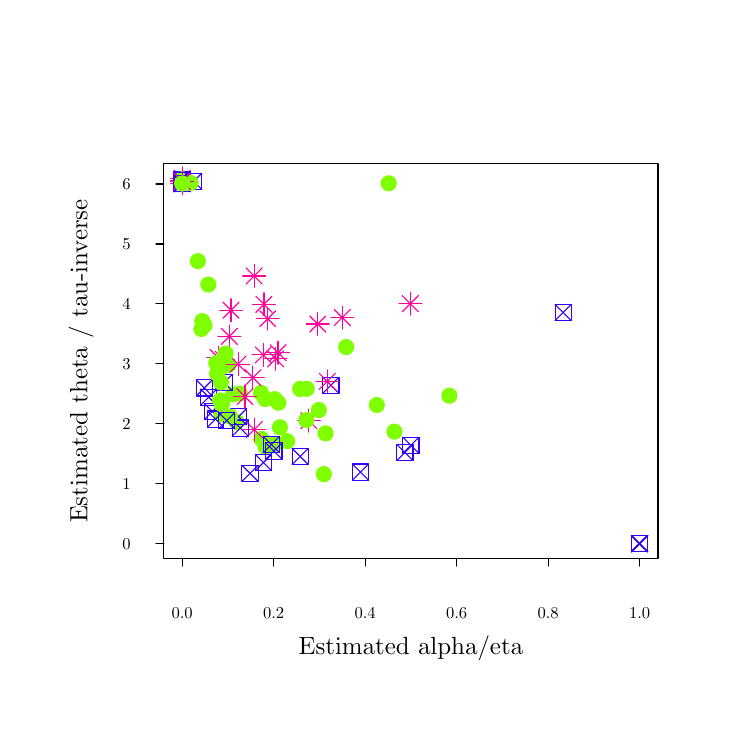
\begin{tikzpicture}[x=1pt,y=1pt]
\definecolor{fillColor}{RGB}{255,255,255}
\path[use as bounding box,fill=fillColor,fill opacity=0.00] (0,0) rectangle (252.94,252.94);
\begin{scope}
\path[clip] ( 49.20, 61.20) rectangle (227.75,203.75);
\definecolor{fillColor}{RGB}{128,255,0}

\path[fill=fillColor] ( 65.27,160.12) circle (  2.92);
\definecolor{drawColor}{RGB}{255,0,153}

\path[draw=drawColor,line width= 0.4pt,line join=round,line cap=round] ( 67.72,130.20) -- ( 73.57,136.05);

\path[draw=drawColor,line width= 0.4pt,line join=round,line cap=round] ( 67.72,136.05) -- ( 73.57,130.20);

\path[draw=drawColor,line width= 0.4pt,line join=round,line cap=round] ( 66.51,133.12) -- ( 74.79,133.12);

\path[draw=drawColor,line width= 0.4pt,line join=round,line cap=round] ( 70.65,128.99) -- ( 70.65,137.26);
\definecolor{drawColor}{RGB}{51,0,255}

\path[draw=drawColor,line width= 0.4pt,line join=round,line cap=round] (218.21, 63.55) rectangle (224.06, 69.40);

\path[draw=drawColor,line width= 0.4pt,line join=round,line cap=round] (218.21, 63.55) -- (224.06, 69.40);

\path[draw=drawColor,line width= 0.4pt,line join=round,line cap=round] (218.21, 69.40) -- (224.06, 63.55);

\path[draw=drawColor,line width= 0.4pt,line join=round,line cap=round] (106.64,120.80) rectangle (112.49,126.65);

\path[draw=drawColor,line width= 0.4pt,line join=round,line cap=round] (106.64,120.80) -- (112.49,126.65);

\path[draw=drawColor,line width= 0.4pt,line join=round,line cap=round] (106.64,126.65) -- (112.49,120.80);

\path[fill=fillColor] ( 84.30,120.99) circle (  2.92);

\path[draw=drawColor,line width= 0.4pt,line join=round,line cap=round] ( 60.90,119.83) rectangle ( 66.75,125.68);

\path[draw=drawColor,line width= 0.4pt,line join=round,line cap=round] ( 60.90,119.83) -- ( 66.75,125.68);

\path[draw=drawColor,line width= 0.4pt,line join=round,line cap=round] ( 60.90,125.68) -- ( 66.75,119.83);

\path[fill=fillColor] ( 89.36,102.57) circle (  2.92);

\path[fill=fillColor] (130.46,196.70) circle (  2.92);

\path[fill=fillColor] ( 90.59,117.40) circle (  2.92);
\definecolor{drawColor}{RGB}{255,0,153}

\path[draw=drawColor,line width= 0.4pt,line join=round,line cap=round] ( 65.90,130.77) -- ( 71.75,136.62);

\path[draw=drawColor,line width= 0.4pt,line join=round,line cap=round] ( 65.90,136.62) -- ( 71.75,130.77);

\path[draw=drawColor,line width= 0.4pt,line join=round,line cap=round] ( 64.69,133.69) -- ( 72.96,133.69);

\path[draw=drawColor,line width= 0.4pt,line join=round,line cap=round] ( 68.83,129.56) -- ( 68.83,137.83);

\path[fill=fillColor] ( 55.81,197.41) circle (  2.92);

\path[fill=fillColor] ( 84.47,104.36) circle (  2.92);

\path[fill=fillColor] ( 56.45,197.12) circle (  2.92);

\path[fill=fillColor] ( 74.23,120.45) circle (  2.92);
\definecolor{drawColor}{RGB}{51,0,255}

\path[draw=drawColor,line width= 0.4pt,line join=round,line cap=round] ( 52.89,194.63) rectangle ( 58.74,200.48);

\path[draw=drawColor,line width= 0.4pt,line join=round,line cap=round] ( 52.89,194.63) -- ( 58.74,200.48);

\path[draw=drawColor,line width= 0.4pt,line join=round,line cap=round] ( 52.89,200.48) -- ( 58.74,194.63);

\path[draw=drawColor,line width= 0.4pt,line join=round,line cap=round] ( 52.89,194.60) rectangle ( 58.74,200.45);

\path[draw=drawColor,line width= 0.4pt,line join=round,line cap=round] ( 52.89,194.60) -- ( 58.74,200.45);

\path[draw=drawColor,line width= 0.4pt,line join=round,line cap=round] ( 52.89,200.45) -- ( 58.74,194.60);
\definecolor{drawColor}{RGB}{255,0,153}

\path[draw=drawColor,line width= 0.4pt,line join=round,line cap=round] (101.89,142.93) -- (107.74,148.78);

\path[draw=drawColor,line width= 0.4pt,line join=round,line cap=round] (101.89,148.78) -- (107.74,142.93);

\path[draw=drawColor,line width= 0.4pt,line join=round,line cap=round] (100.68,145.86) -- (108.95,145.86);

\path[draw=drawColor,line width= 0.4pt,line join=round,line cap=round] (104.82,141.72) -- (104.82,149.99);
\definecolor{drawColor}{RGB}{51,0,255}

\path[draw=drawColor,line width= 0.4pt,line join=round,line cap=round] ( 62.47,116.50) rectangle ( 68.32,122.35);

\path[draw=drawColor,line width= 0.4pt,line join=round,line cap=round] ( 62.47,116.50) -- ( 68.32,122.35);

\path[draw=drawColor,line width= 0.4pt,line join=round,line cap=round] ( 62.47,122.35) -- ( 68.32,116.50);
\definecolor{drawColor}{RGB}{255,0,153}

\path[draw=drawColor,line width= 0.4pt,line join=round,line cap=round] ( 98.67,108.01) -- (104.52,113.86);

\path[draw=drawColor,line width= 0.4pt,line join=round,line cap=round] ( 98.67,113.86) -- (104.52,108.01);

\path[draw=drawColor,line width= 0.4pt,line join=round,line cap=round] ( 97.45,110.93) -- (105.73,110.93);

\path[draw=drawColor,line width= 0.4pt,line join=round,line cap=round] (101.59,106.80) -- (101.59,115.07);
\definecolor{drawColor}{RGB}{51,0,255}

\path[draw=drawColor,line width= 0.4pt,line join=round,line cap=round] ( 52.89,193.75) rectangle ( 58.74,199.60);

\path[draw=drawColor,line width= 0.4pt,line join=round,line cap=round] ( 52.89,193.75) -- ( 58.74,199.60);

\path[draw=drawColor,line width= 0.4pt,line join=round,line cap=round] ( 52.89,199.60) -- ( 58.74,193.75);

\path[draw=drawColor,line width= 0.4pt,line join=round,line cap=round] (218.09, 63.55) rectangle (223.94, 69.40);

\path[draw=drawColor,line width= 0.4pt,line join=round,line cap=round] (218.09, 63.55) -- (223.94, 69.40);

\path[draw=drawColor,line width= 0.4pt,line join=round,line cap=round] (218.09, 69.40) -- (223.94, 63.55);

\path[fill=fillColor] ( 76.68,120.70) circle (  2.92);

\path[fill=fillColor] ( 69.50,129.74) circle (  2.92);
\definecolor{drawColor}{RGB}{255,0,153}

\path[draw=drawColor,line width= 0.4pt,line join=round,line cap=round] ( 52.89,195.54) -- ( 58.74,201.39);

\path[draw=drawColor,line width= 0.4pt,line join=round,line cap=round] ( 52.89,201.39) -- ( 58.74,195.54);

\path[draw=drawColor,line width= 0.4pt,line join=round,line cap=round] ( 51.68,198.47) -- ( 59.95,198.47);

\path[draw=drawColor,line width= 0.4pt,line join=round,line cap=round] ( 55.81,194.33) -- ( 55.81,202.60);
\definecolor{drawColor}{RGB}{51,0,255}

\path[draw=drawColor,line width= 0.4pt,line join=round,line cap=round] ( 63.79,111.31) rectangle ( 69.64,117.16);

\path[draw=drawColor,line width= 0.4pt,line join=round,line cap=round] ( 63.79,111.31) -- ( 69.64,117.16);

\path[draw=drawColor,line width= 0.4pt,line join=round,line cap=round] ( 63.79,117.16) -- ( 69.64,111.31);
\definecolor{drawColor}{RGB}{255,0,153}

\path[draw=drawColor,line width= 0.4pt,line join=round,line cap=round] ( 52.89,194.66) -- ( 58.74,200.51);

\path[draw=drawColor,line width= 0.4pt,line join=round,line cap=round] ( 52.89,200.51) -- ( 58.74,194.66);

\path[draw=drawColor,line width= 0.4pt,line join=round,line cap=round] ( 51.68,197.59) -- ( 59.95,197.59);

\path[draw=drawColor,line width= 0.4pt,line join=round,line cap=round] ( 55.81,193.45) -- ( 55.81,201.73);

\path[fill=fillColor] ( 61.52,168.59) circle (  2.92);
\definecolor{drawColor}{RGB}{51,0,255}

\path[draw=drawColor,line width= 0.4pt,line join=round,line cap=round] (218.21, 63.55) rectangle (224.06, 69.40);

\path[draw=drawColor,line width= 0.4pt,line join=round,line cap=round] (218.21, 63.55) -- (224.06, 69.40);

\path[draw=drawColor,line width= 0.4pt,line join=round,line cap=round] (218.21, 69.40) -- (224.06, 63.55);

\path[fill=fillColor] ( 63.90,145.41) circle (  2.92);

\path[fill=fillColor] ( 89.26,118.70) circle (  2.92);
\definecolor{drawColor}{RGB}{255,0,153}

\path[draw=drawColor,line width= 0.4pt,line join=round,line cap=round] ( 78.46,123.54) -- ( 84.31,129.39);

\path[draw=drawColor,line width= 0.4pt,line join=round,line cap=round] ( 78.46,129.39) -- ( 84.31,123.54);

\path[draw=drawColor,line width= 0.4pt,line join=round,line cap=round] ( 77.24,126.46) -- ( 85.52,126.46);

\path[draw=drawColor,line width= 0.4pt,line join=round,line cap=round] ( 81.38,122.33) -- ( 81.38,130.60);

\path[fill=fillColor] ( 75.51,110.46) circle (  2.92);

\path[fill=fillColor] ( 85.88,101.53) circle (  2.92);

\path[draw=drawColor,line width= 0.4pt,line join=round,line cap=round] ( 69.96,138.46) -- ( 75.81,144.31);

\path[draw=drawColor,line width= 0.4pt,line join=round,line cap=round] ( 69.96,144.31) -- ( 75.81,138.46);

\path[draw=drawColor,line width= 0.4pt,line join=round,line cap=round] ( 68.75,141.38) -- ( 77.03,141.38);

\path[draw=drawColor,line width= 0.4pt,line join=round,line cap=round] ( 72.89,137.24) -- ( 72.89,145.52);

\path[fill=fillColor] (107.02, 91.62) circle (  2.92);
\definecolor{drawColor}{RGB}{51,0,255}

\path[draw=drawColor,line width= 0.4pt,line join=round,line cap=round] (218.21, 63.55) rectangle (224.06, 69.40);

\path[draw=drawColor,line width= 0.4pt,line join=round,line cap=round] (218.21, 63.55) -- (224.06, 69.40);

\path[draw=drawColor,line width= 0.4pt,line join=round,line cap=round] (218.21, 69.40) -- (224.06, 63.55);

\path[fill=fillColor] (105.22,114.77) circle (  2.92);

\path[draw=drawColor,line width= 0.4pt,line join=round,line cap=round] ( 52.89,195.12) rectangle ( 58.74,200.97);

\path[draw=drawColor,line width= 0.4pt,line join=round,line cap=round] ( 52.89,195.12) -- ( 58.74,200.97);

\path[draw=drawColor,line width= 0.4pt,line join=round,line cap=round] ( 52.89,200.97) -- ( 58.74,195.12);

\path[draw=drawColor,line width= 0.4pt,line join=round,line cap=round] (117.35, 89.42) rectangle (123.20, 95.27);

\path[draw=drawColor,line width= 0.4pt,line join=round,line cap=round] (117.35, 89.42) -- (123.20, 95.27);

\path[draw=drawColor,line width= 0.4pt,line join=round,line cap=round] (117.35, 95.27) -- (123.20, 89.42);

\path[draw=drawColor,line width= 0.4pt,line join=round,line cap=round] (133.40, 96.50) rectangle (139.25,102.35);

\path[draw=drawColor,line width= 0.4pt,line join=round,line cap=round] (133.40, 96.50) -- (139.25,102.35);

\path[draw=drawColor,line width= 0.4pt,line join=round,line cap=round] (133.40,102.35) -- (139.25, 96.50);

\path[draw=drawColor,line width= 0.4pt,line join=round,line cap=round] ( 68.06,121.82) rectangle ( 73.91,127.67);

\path[draw=drawColor,line width= 0.4pt,line join=round,line cap=round] ( 68.06,121.82) -- ( 73.91,127.67);

\path[draw=drawColor,line width= 0.4pt,line join=round,line cap=round] ( 68.06,127.67) -- ( 73.91,121.82);

\path[fill=fillColor] ( 72.52,131.03) circle (  2.92);

\path[draw=drawColor,line width= 0.4pt,line join=round,line cap=round] ( 52.89,194.32) rectangle ( 58.74,200.17);

\path[draw=drawColor,line width= 0.4pt,line join=round,line cap=round] ( 52.89,194.32) -- ( 58.74,200.17);

\path[draw=drawColor,line width= 0.4pt,line join=round,line cap=round] ( 52.89,200.17) -- ( 58.74,194.32);

\path[draw=drawColor,line width= 0.4pt,line join=round,line cap=round] ( 52.89,195.15) rectangle ( 58.74,201.00);

\path[draw=drawColor,line width= 0.4pt,line join=round,line cap=round] ( 52.89,195.15) -- ( 58.74,201.00);

\path[draw=drawColor,line width= 0.4pt,line join=round,line cap=round] ( 52.89,201.00) -- ( 58.74,195.15);
\definecolor{drawColor}{RGB}{255,0,153}

\path[draw=drawColor,line width= 0.4pt,line join=round,line cap=round] ( 73.09,128.44) -- ( 78.94,134.29);

\path[draw=drawColor,line width= 0.4pt,line join=round,line cap=round] ( 73.09,134.29) -- ( 78.94,128.44);

\path[draw=drawColor,line width= 0.4pt,line join=round,line cap=round] ( 71.88,131.37) -- ( 80.16,131.37);

\path[draw=drawColor,line width= 0.4pt,line join=round,line cap=round] ( 76.02,127.23) -- ( 76.02,135.50);

\path[fill=fillColor] ( 93.76,103.53) circle (  2.92);

\path[draw=drawColor,line width= 0.4pt,line join=round,line cap=round] ( 86.70,130.32) -- ( 92.55,136.17);

\path[draw=drawColor,line width= 0.4pt,line join=round,line cap=round] ( 86.70,136.17) -- ( 92.55,130.32);

\path[draw=drawColor,line width= 0.4pt,line join=round,line cap=round] ( 85.48,133.25) -- ( 93.76,133.25);

\path[draw=drawColor,line width= 0.4pt,line join=round,line cap=round] ( 89.62,129.11) -- ( 89.62,137.38);

\path[draw=drawColor,line width= 0.4pt,line join=round,line cap=round] (135.34,150.28) -- (141.19,156.13);

\path[draw=drawColor,line width= 0.4pt,line join=round,line cap=round] (135.34,156.13) -- (141.19,150.28);

\path[draw=drawColor,line width= 0.4pt,line join=round,line cap=round] (134.13,153.21) -- (142.41,153.21);

\path[draw=drawColor,line width= 0.4pt,line join=round,line cap=round] (138.27,149.07) -- (138.27,157.34);

\path[fill=fillColor] (126.16,116.59) circle (  2.92);
\definecolor{drawColor}{RGB}{51,0,255}

\path[draw=drawColor,line width= 0.4pt,line join=round,line cap=round] ( 52.89,195.02) rectangle ( 58.74,200.87);

\path[draw=drawColor,line width= 0.4pt,line join=round,line cap=round] ( 52.89,195.02) -- ( 58.74,200.87);

\path[draw=drawColor,line width= 0.4pt,line join=round,line cap=round] ( 52.89,200.87) -- ( 58.74,195.02);
\definecolor{drawColor}{RGB}{255,0,153}

\path[draw=drawColor,line width= 0.4pt,line join=round,line cap=round] ( 78.90,160.29) -- ( 84.75,166.14);

\path[draw=drawColor,line width= 0.4pt,line join=round,line cap=round] ( 78.90,166.14) -- ( 84.75,160.29);

\path[draw=drawColor,line width= 0.4pt,line join=round,line cap=round] ( 77.69,163.22) -- ( 85.96,163.22);

\path[draw=drawColor,line width= 0.4pt,line join=round,line cap=round] ( 81.83,159.08) -- ( 81.83,167.36);

\path[fill=fillColor] ( 70.07,113.18) circle (  2.92);

\path[fill=fillColor] ( 55.81,198.16) circle (  2.92);

\path[draw=drawColor,line width= 0.4pt,line join=round,line cap=round] (105.35,122.20) -- (111.20,128.05);

\path[draw=drawColor,line width= 0.4pt,line join=round,line cap=round] (105.35,128.05) -- (111.20,122.20);

\path[draw=drawColor,line width= 0.4pt,line join=round,line cap=round] (104.14,125.13) -- (112.41,125.13);

\path[draw=drawColor,line width= 0.4pt,line join=round,line cap=round] (108.27,120.99) -- (108.27,129.26);
\definecolor{drawColor}{RGB}{51,0,255}

\path[draw=drawColor,line width= 0.4pt,line join=round,line cap=round] (190.58,147.10) rectangle (196.43,152.95);

\path[draw=drawColor,line width= 0.4pt,line join=round,line cap=round] (190.58,147.10) -- (196.43,152.95);

\path[draw=drawColor,line width= 0.4pt,line join=round,line cap=round] (190.58,152.95) -- (196.43,147.10);

\path[draw=drawColor,line width= 0.4pt,line join=round,line cap=round] ( 52.89,193.58) rectangle ( 58.74,199.43);

\path[draw=drawColor,line width= 0.4pt,line join=round,line cap=round] ( 52.89,193.58) -- ( 58.74,199.43);

\path[draw=drawColor,line width= 0.4pt,line join=round,line cap=round] ( 52.89,199.43) -- ( 58.74,193.58);

\path[draw=drawColor,line width= 0.4pt,line join=round,line cap=round] ( 82.27, 92.88) rectangle ( 88.12, 98.73);

\path[draw=drawColor,line width= 0.4pt,line join=round,line cap=round] ( 82.27, 92.88) -- ( 88.12, 98.73);

\path[draw=drawColor,line width= 0.4pt,line join=round,line cap=round] ( 82.27, 98.73) -- ( 88.12, 92.88);

\path[fill=fillColor] ( 62.77,144.08) circle (  2.92);

\path[draw=drawColor,line width= 0.4pt,line join=round,line cap=round] ( 57.06,194.49) rectangle ( 62.91,200.34);

\path[draw=drawColor,line width= 0.4pt,line join=round,line cap=round] ( 57.06,194.49) -- ( 62.91,200.34);

\path[draw=drawColor,line width= 0.4pt,line join=round,line cap=round] ( 57.06,200.34) -- ( 62.91,194.49);

\path[draw=drawColor,line width= 0.4pt,line join=round,line cap=round] (218.21, 63.55) rectangle (224.06, 69.40);

\path[draw=drawColor,line width= 0.4pt,line join=round,line cap=round] (218.21, 63.55) -- (224.06, 69.40);

\path[draw=drawColor,line width= 0.4pt,line join=round,line cap=round] (218.21, 69.40) -- (224.06, 63.55);
\definecolor{drawColor}{RGB}{255,0,153}

\path[draw=drawColor,line width= 0.4pt,line join=round,line cap=round] ( 87.54,132.55) -- ( 93.39,138.40);

\path[draw=drawColor,line width= 0.4pt,line join=round,line cap=round] ( 87.54,138.40) -- ( 93.39,132.55);

\path[draw=drawColor,line width= 0.4pt,line join=round,line cap=round] ( 86.33,135.47) -- ( 94.60,135.47);

\path[draw=drawColor,line width= 0.4pt,line join=round,line cap=round] ( 90.47,131.34) -- ( 90.47,139.61);
\definecolor{drawColor}{RGB}{51,0,255}

\path[draw=drawColor,line width= 0.4pt,line join=round,line cap=round] ( 86.04, 97.03) rectangle ( 91.89,102.88);

\path[draw=drawColor,line width= 0.4pt,line join=round,line cap=round] ( 86.04, 97.03) -- ( 91.89,102.88);

\path[draw=drawColor,line width= 0.4pt,line join=round,line cap=round] ( 86.04,102.88) -- ( 91.89, 97.03);

\path[draw=drawColor,line width= 0.4pt,line join=round,line cap=round] ( 77.42, 88.99) rectangle ( 83.27, 94.84);

\path[draw=drawColor,line width= 0.4pt,line join=round,line cap=round] ( 77.42, 88.99) -- ( 83.27, 94.84);

\path[draw=drawColor,line width= 0.4pt,line join=round,line cap=round] ( 77.42, 94.84) -- ( 83.27, 88.99);

\path[draw=drawColor,line width= 0.4pt,line join=round,line cap=round] (218.09, 63.55) rectangle (223.94, 69.40);

\path[draw=drawColor,line width= 0.4pt,line join=round,line cap=round] (218.09, 63.55) -- (223.94, 69.40);

\path[draw=drawColor,line width= 0.4pt,line join=round,line cap=round] (218.09, 69.40) -- (223.94, 63.55);

\path[draw=drawColor,line width= 0.4pt,line join=round,line cap=round] ( 73.26,109.43) rectangle ( 79.11,115.28);

\path[draw=drawColor,line width= 0.4pt,line join=round,line cap=round] ( 73.26,109.43) -- ( 79.11,115.28);

\path[draw=drawColor,line width= 0.4pt,line join=round,line cap=round] ( 73.26,115.28) -- ( 79.11,109.43);

\path[fill=fillColor] ( 91.14,108.55) circle (  2.92);

\path[fill=fillColor] ( 85.77,118.76) circle (  2.92);
\definecolor{drawColor}{RGB}{255,0,153}

\path[draw=drawColor,line width= 0.4pt,line join=round,line cap=round] ( 52.89,193.74) -- ( 58.74,199.59);

\path[draw=drawColor,line width= 0.4pt,line join=round,line cap=round] ( 52.89,199.59) -- ( 58.74,193.74);

\path[draw=drawColor,line width= 0.4pt,line join=round,line cap=round] ( 51.68,196.67) -- ( 59.95,196.67);

\path[draw=drawColor,line width= 0.4pt,line join=round,line cap=round] ( 55.81,192.53) -- ( 55.81,200.80);

\path[fill=fillColor] (100.83,122.44) circle (  2.92);

\path[draw=drawColor,line width= 0.4pt,line join=round,line cap=round] ( 78.97,104.76) -- ( 84.82,110.61);

\path[draw=drawColor,line width= 0.4pt,line join=round,line cap=round] ( 78.97,110.61) -- ( 84.82,104.76);

\path[draw=drawColor,line width= 0.4pt,line join=round,line cap=round] ( 77.75,107.68) -- ( 86.03,107.68);

\path[draw=drawColor,line width= 0.4pt,line join=round,line cap=round] ( 81.89,103.55) -- ( 81.89,111.82);
\definecolor{drawColor}{RGB}{51,0,255}

\path[draw=drawColor,line width= 0.4pt,line join=round,line cap=round] ( 73.91,105.31) rectangle ( 79.76,111.16);

\path[draw=drawColor,line width= 0.4pt,line join=round,line cap=round] ( 73.91,105.31) -- ( 79.76,111.16);

\path[draw=drawColor,line width= 0.4pt,line join=round,line cap=round] ( 73.91,111.16) -- ( 79.76,105.31);
\definecolor{drawColor}{RGB}{255,0,153}

\path[draw=drawColor,line width= 0.4pt,line join=round,line cap=round] ( 83.83,144.83) -- ( 89.68,150.68);

\path[draw=drawColor,line width= 0.4pt,line join=round,line cap=round] ( 83.83,150.68) -- ( 89.68,144.83);

\path[draw=drawColor,line width= 0.4pt,line join=round,line cap=round] ( 82.62,147.75) -- ( 90.89,147.75);

\path[draw=drawColor,line width= 0.4pt,line join=round,line cap=round] ( 86.75,143.62) -- ( 86.75,151.89);

\path[fill=fillColor] ( 98.44,122.39) circle (  2.92);

\path[draw=drawColor,line width= 0.4pt,line join=round,line cap=round] ( 75.60,116.66) -- ( 81.45,122.51);

\path[draw=drawColor,line width= 0.4pt,line join=round,line cap=round] ( 75.60,122.51) -- ( 81.45,116.66);

\path[draw=drawColor,line width= 0.4pt,line join=round,line cap=round] ( 74.39,119.58) -- ( 82.66,119.58);

\path[draw=drawColor,line width= 0.4pt,line join=round,line cap=round] ( 78.53,115.45) -- ( 78.53,123.72);

\path[fill=fillColor] (115.09,137.54) circle (  2.92);
\definecolor{drawColor}{RGB}{51,0,255}

\path[draw=drawColor,line width= 0.4pt,line join=round,line cap=round] ( 52.89,193.82) rectangle ( 58.74,199.67);

\path[draw=drawColor,line width= 0.4pt,line join=round,line cap=round] ( 52.89,193.82) -- ( 58.74,199.67);

\path[draw=drawColor,line width= 0.4pt,line join=round,line cap=round] ( 52.89,199.67) -- ( 58.74,193.82);

\path[draw=drawColor,line width= 0.4pt,line join=round,line cap=round] (135.56, 99.11) rectangle (141.41,104.96);

\path[draw=drawColor,line width= 0.4pt,line join=round,line cap=round] (135.56, 99.11) -- (141.41,104.96);

\path[draw=drawColor,line width= 0.4pt,line join=round,line cap=round] (135.56,104.96) -- (141.41, 99.11);

\path[draw=drawColor,line width= 0.4pt,line join=round,line cap=round] ( 64.94,108.57) rectangle ( 70.79,114.42);

\path[draw=drawColor,line width= 0.4pt,line join=round,line cap=round] ( 64.94,108.57) -- ( 70.79,114.42);

\path[draw=drawColor,line width= 0.4pt,line join=round,line cap=round] ( 64.94,114.42) -- ( 70.79,108.57);
\definecolor{drawColor}{RGB}{255,0,153}

\path[draw=drawColor,line width= 0.4pt,line join=round,line cap=round] ( 70.55,147.91) -- ( 76.40,153.76);

\path[draw=drawColor,line width= 0.4pt,line join=round,line cap=round] ( 70.55,153.76) -- ( 76.40,147.91);

\path[draw=drawColor,line width= 0.4pt,line join=round,line cap=round] ( 69.34,150.84) -- ( 77.61,150.84);

\path[draw=drawColor,line width= 0.4pt,line join=round,line cap=round] ( 73.48,146.70) -- ( 73.48,154.97);
\definecolor{drawColor}{RGB}{51,0,255}

\path[draw=drawColor,line width= 0.4pt,line join=round,line cap=round] ( 52.89,194.62) rectangle ( 58.74,200.47);

\path[draw=drawColor,line width= 0.4pt,line join=round,line cap=round] ( 52.89,194.62) -- ( 58.74,200.47);

\path[draw=drawColor,line width= 0.4pt,line join=round,line cap=round] ( 52.89,200.47) -- ( 58.74,194.62);

\path[fill=fillColor] ( 73.17,112.39) circle (  2.92);

\path[fill=fillColor] ( 68.14,131.73) circle (  2.92);
\definecolor{drawColor}{RGB}{255,0,153}

\path[draw=drawColor,line width= 0.4pt,line join=round,line cap=round] ( 82.22,131.78) -- ( 88.07,137.63);

\path[draw=drawColor,line width= 0.4pt,line join=round,line cap=round] ( 82.22,137.63) -- ( 88.07,131.78);

\path[draw=drawColor,line width= 0.4pt,line join=round,line cap=round] ( 81.01,134.71) -- ( 89.29,134.71);

\path[draw=drawColor,line width= 0.4pt,line join=round,line cap=round] ( 85.15,130.57) -- ( 85.15,138.84);

\path[fill=fillColor] ( 58.88,196.84) circle (  2.92);

\path[draw=drawColor,line width= 0.4pt,line join=round,line cap=round] ( 52.89,194.48) -- ( 58.74,200.33);

\path[draw=drawColor,line width= 0.4pt,line join=round,line cap=round] ( 52.89,200.33) -- ( 58.74,194.48);

\path[draw=drawColor,line width= 0.4pt,line join=round,line cap=round] ( 51.68,197.41) -- ( 59.95,197.41);

\path[draw=drawColor,line width= 0.4pt,line join=round,line cap=round] ( 55.81,193.27) -- ( 55.81,201.54);

\path[fill=fillColor] ( 55.81,196.63) circle (  2.92);

\path[fill=fillColor] ( 70.18,116.89) circle (  2.92);
\definecolor{drawColor}{RGB}{51,0,255}

\path[draw=drawColor,line width= 0.4pt,line join=round,line cap=round] ( 85.13, 99.39) rectangle ( 90.98,105.24);

\path[draw=drawColor,line width= 0.4pt,line join=round,line cap=round] ( 85.13, 99.39) -- ( 90.98,105.24);

\path[draw=drawColor,line width= 0.4pt,line join=round,line cap=round] ( 85.13,105.24) -- ( 90.98, 99.39);

\path[fill=fillColor] (132.53,106.98) circle (  2.92);

\path[fill=fillColor] (107.64,106.34) circle (  2.92);

\path[fill=fillColor] ( 71.51,135.19) circle (  2.92);
\definecolor{drawColor}{RGB}{255,0,153}

\path[draw=drawColor,line width= 0.4pt,line join=round,line cap=round] ( 82.46,150.05) -- ( 88.31,155.90);

\path[draw=drawColor,line width= 0.4pt,line join=round,line cap=round] ( 82.46,155.90) -- ( 88.31,150.05);

\path[draw=drawColor,line width= 0.4pt,line join=round,line cap=round] ( 81.25,152.98) -- ( 89.52,152.98);

\path[draw=drawColor,line width= 0.4pt,line join=round,line cap=round] ( 85.38,148.84) -- ( 85.38,157.12);
\definecolor{drawColor}{RGB}{51,0,255}

\path[draw=drawColor,line width= 0.4pt,line join=round,line cap=round] ( 69.01,108.04) rectangle ( 74.86,113.89);

\path[draw=drawColor,line width= 0.4pt,line join=round,line cap=round] ( 69.01,108.04) -- ( 74.86,113.89);

\path[draw=drawColor,line width= 0.4pt,line join=round,line cap=round] ( 69.01,113.89) -- ( 74.86,108.04);
\definecolor{drawColor}{RGB}{255,0,153}

\path[draw=drawColor,line width= 0.4pt,line join=round,line cap=round] (110.76,145.26) -- (116.61,151.11);

\path[draw=drawColor,line width= 0.4pt,line join=round,line cap=round] (110.76,151.11) -- (116.61,145.26);

\path[draw=drawColor,line width= 0.4pt,line join=round,line cap=round] (109.55,148.19) -- (117.82,148.19);

\path[draw=drawColor,line width= 0.4pt,line join=round,line cap=round] (113.68,144.05) -- (113.68,152.33);

\path[fill=fillColor] ( 63.09,146.93) circle (  2.92);

\path[fill=fillColor] ( 69.53,118.25) circle (  2.92);
\definecolor{drawColor}{RGB}{51,0,255}

\path[draw=drawColor,line width= 0.4pt,line join=round,line cap=round] ( 95.54, 95.09) rectangle (101.39,100.94);

\path[draw=drawColor,line width= 0.4pt,line join=round,line cap=round] ( 95.54, 95.09) -- (101.39,100.94);

\path[draw=drawColor,line width= 0.4pt,line join=round,line cap=round] ( 95.54,100.94) -- (101.39, 95.09);

\path[fill=fillColor] (100.71,111.17) circle (  2.92);

\path[fill=fillColor] (152.38,119.95) circle (  2.92);

\path[fill=fillColor] ( 68.44,127.90) circle (  2.92);

\path[fill=fillColor] ( 69.83,124.75) circle (  2.92);
\end{scope}
\begin{scope}
\path[clip] (  0.00,  0.00) rectangle (252.94,252.94);
\definecolor{drawColor}{RGB}{0,0,0}

\path[draw=drawColor,line width= 0.4pt,line join=round,line cap=round] ( 55.81, 61.20) -- (221.13, 61.20);

\path[draw=drawColor,line width= 0.4pt,line join=round,line cap=round] ( 55.81, 61.20) -- ( 55.81, 58.35);

\path[draw=drawColor,line width= 0.4pt,line join=round,line cap=round] ( 88.88, 61.20) -- ( 88.88, 58.35);

\path[draw=drawColor,line width= 0.4pt,line join=round,line cap=round] (121.94, 61.20) -- (121.94, 58.35);

\path[draw=drawColor,line width= 0.4pt,line join=round,line cap=round] (155.00, 61.20) -- (155.00, 58.35);

\path[draw=drawColor,line width= 0.4pt,line join=round,line cap=round] (188.07, 61.20) -- (188.07, 58.35);

\path[draw=drawColor,line width= 0.4pt,line join=round,line cap=round] (221.13, 61.20) -- (221.13, 58.35);

\node[text=drawColor,anchor=base,inner sep=0pt, outer sep=0pt, scale=  0.60] at ( 55.81, 39.60) {0.0};

\node[text=drawColor,anchor=base,inner sep=0pt, outer sep=0pt, scale=  0.60] at ( 88.88, 39.60) {0.2};

\node[text=drawColor,anchor=base,inner sep=0pt, outer sep=0pt, scale=  0.60] at (121.94, 39.60) {0.4};

\node[text=drawColor,anchor=base,inner sep=0pt, outer sep=0pt, scale=  0.60] at (155.00, 39.60) {0.6};

\node[text=drawColor,anchor=base,inner sep=0pt, outer sep=0pt, scale=  0.60] at (188.07, 39.60) {0.8};

\node[text=drawColor,anchor=base,inner sep=0pt, outer sep=0pt, scale=  0.60] at (221.13, 39.60) {1.0};

\path[draw=drawColor,line width= 0.4pt,line join=round,line cap=round] ( 49.20, 66.48) -- ( 49.20,196.44);

\path[draw=drawColor,line width= 0.4pt,line join=round,line cap=round] ( 49.20, 66.48) -- ( 46.35, 66.48);

\path[draw=drawColor,line width= 0.4pt,line join=round,line cap=round] ( 49.20, 88.14) -- ( 46.35, 88.14);

\path[draw=drawColor,line width= 0.4pt,line join=round,line cap=round] ( 49.20,109.80) -- ( 46.35,109.80);

\path[draw=drawColor,line width= 0.4pt,line join=round,line cap=round] ( 49.20,131.46) -- ( 46.35,131.46);

\path[draw=drawColor,line width= 0.4pt,line join=round,line cap=round] ( 49.20,153.12) -- ( 46.35,153.12);

\path[draw=drawColor,line width= 0.4pt,line join=round,line cap=round] ( 49.20,174.78) -- ( 46.35,174.78);

\path[draw=drawColor,line width= 0.4pt,line join=round,line cap=round] ( 49.20,196.44) -- ( 46.35,196.44);

\node[text=drawColor,anchor=base east,inner sep=0pt, outer sep=0pt, scale=  0.60] at ( 37.20, 64.41) {0};

\node[text=drawColor,anchor=base east,inner sep=0pt, outer sep=0pt, scale=  0.60] at ( 37.20, 86.07) {1};

\node[text=drawColor,anchor=base east,inner sep=0pt, outer sep=0pt, scale=  0.60] at ( 37.20,107.73) {2};

\node[text=drawColor,anchor=base east,inner sep=0pt, outer sep=0pt, scale=  0.60] at ( 37.20,129.40) {3};

\node[text=drawColor,anchor=base east,inner sep=0pt, outer sep=0pt, scale=  0.60] at ( 37.20,151.06) {4};

\node[text=drawColor,anchor=base east,inner sep=0pt, outer sep=0pt, scale=  0.60] at ( 37.20,172.72) {5};

\node[text=drawColor,anchor=base east,inner sep=0pt, outer sep=0pt, scale=  0.60] at ( 37.20,194.38) {6};

\path[draw=drawColor,line width= 0.4pt,line join=round,line cap=round] ( 49.20, 61.20) --
	(227.75, 61.20) --
	(227.75,203.75) --
	( 49.20,203.75) --
	( 49.20, 61.20);
\end{scope}
\begin{scope}
\path[clip] (  0.00,  0.00) rectangle (252.94,252.94);
\definecolor{drawColor}{RGB}{0,0,0}

\node[text=drawColor,anchor=base,inner sep=0pt, outer sep=0pt, scale=  0.90] at (138.47, 26.40) {Estimated alpha/eta};

\node[text=drawColor,rotate= 90.00,anchor=base,inner sep=0pt, outer sep=0pt, scale=  0.90] at ( 21.60,132.47) {Estimated theta / tau-inverse};
\end{scope}
\end{tikzpicture}

\end{frame}


\begin{frame}{Experiment Results}
	\framesubtitle{IGT data for conviceted criminals}
	\setbeamertemplate{itemize items}[circle]
	Authors results:
	\begin{itemize}
		\item Specialized version IGT test
		\item No control group
		\item EVM analysis shows clustering for convicted robbery and assault/murders; Other criminal groups have overlapping parameters
	\end{itemize}
		Our findings:
		\begin{itemize}
			\item Convicted assault/murders separate the strongest (highest clustering against forgery)
			\item Robbery only cluster moderat in our settings. 
		\end{itemize}
\end{frame}

\begin{frame}{Experiment Results}
	\framesubtitle{IGT data for drug abusers}
	\setbeamertemplate{itemize items}[circle]
	Author's findings
	\begin{itemize}
		\item Cocaine abusers persistently do disadvantageous choices
		\item Effect still present after controlling for IQ (in general lower than within control group)
	\end{itemize}
	Our findings
	\begin{itemize}
		\item Only moderate clustering between control group and cocaine abusers
		\item Best septation criteria turned out disadvantageous behaviour
	\end{itemize}
\end{frame}


\begin{frame}{Conclusion}
	\setbeamertemplate{itemize items}[circle]
	Key - Finings
	\begin{itemize}
		\item Clustering peoples choices in general difficult
		\item Algorithms can recover clustering if individuals show sufficient difference in their strategic behaviour
		\item Other studies found a strong attention to gains and no learning from negative experience
	\end{itemize}
	
\end{frame}

\end{document}